\documentclass{article}

\usepackage[english]{babel}

\usepackage[letterpaper,top=2cm,bottom=2cm,left=3cm,right=3cm,marginparwidth=1.75cm]{geometry}

% Useful packages
\usepackage{amsmath}
\usepackage{amssymb}
\usepackage{xcolor}
\usepackage{graphicx}
\usepackage{mathtools}
\usepackage{framed}
\usepackage{tikz}
\usepackage[colorlinks=true, allcolors=blue]{hyperref}
\usepackage{xcolor}
\usepackage{colortbl}
\usepackage{booktabs}
\usepackage{tikz}
\usepackage{tcolorbox}
\usepackage{amsthm}
\usepackage[noabbrev]{cleveref}
\usetikzlibrary{positioning, arrows.meta, decorations.pathreplacing}

\theoremstyle{definition}
\newtheorem{exmp}{Example}[section]

\definecolor{sigblue}{RGB}{214,228,247}
\definecolor{siggreen}{RGB}{208,235,203}
\definecolor{sigyellow}{RGB}{255,245,200}

\newcommand{\Fp}{\mathbb F_p}
\newcommand{\Fq}{\mathbb F_q}
\newcommand{\offdest}{\text{off}_{\text{dest}}}
\newcommand{\offopzero}{\text{off}_{\text{op0}}}
\newcommand{\offopone}{\text{off}_{\text{op1}}}
\newcommand*{\logeq}{\ratio\Leftrightarrow}
\newcommand{\nextmle}{\overset{\scriptscriptstyle\wedge}{\textsf{next}}}

\newtheorem{lemma}{Lemma}
\newtheorem{theorem}{Theorem}

\title{LeanVM}
\author{draft 0.8.0 (Work In Progress)}
\date{}
\begin{document}

\maketitle

\tableofcontents
\newpage

\section{Introduction}
Ethereum's cryptography currently relies on elliptic curves, which are known to be vulnerable to quantum computers \cite{shor}.

LeanVM is a verifiable Virtual Machine (also called zkVM for "zero knowledge VM"). It uses a minimal ISA (Instruction Set Architecture) inspired by Cairo \cite{cairo}.
\begin{itemize}
    \item It's hash-based (WHIR \cite{whir}): plausibly post-quantum, conceptually simple
    \item It's multilinear: the trace is committed as a single multilinear polynomial (reducing proof size), and constraints are proven via sumcheck \cite{sumcheck}
    \item It uses the Poseidon \cite{poseidon1} permutation as a snark-friendly hashing primitive
\end{itemize}

\section{Use-cases}

LeanVM is optimized to provide a post-quantum alternative for each of the three layers of Ethereum:

\subsection{Consensus Layer}
\begin{itemize}
    \item \textbf{Currently (pre-quantum):} BLS \cite{bls}: lightweight signatures of 96 bytes, with native support for aggregation.
    \item \textbf{With LeanVM (post-quantum):} Replace BLS by XMSS over Poseidon \cite{ethereum_signatures} (leanXMSS). Aggregate those signatures using leanVM. Already aggregated signatures can be further merged, via recursion. XMSS is a stateful signature scheme, but Ethereum's slot can be used as a nonce (double signing is already prevented).
\end{itemize}

See \Cref{sec:signature-aggregation} for more details.

\subsection{Execution Layer}
\begin{itemize}
    \item \textbf{Currently (pre-quantum):} ECDSA \cite{ecdsa}
    \item \textbf{With LeanVM (post-quantum):} Replace ECDSA by a variant of SPHINCS+ \cite{sphincs_plus} over poseidon (leanSPHINCS). Aggregate all the signatures from one block using leanVM.
\end{itemize}

See \Cref{sec:signature-aggregation} for more details.

\subsection{Data Availability Layer}

\begin{itemize}
    \item \textbf{Currently (pre-quantum):} KZG polynomial commitment scheme \cite{kzg}
    \item \textbf{With LeanVM (post-quantum):} Reed-Solomon encode and Merkle-commit the codeword, for each blob. Prove the claimed Merkle Root was correctly computed using leanVM.
\end{itemize}

\section{Preliminaries}

\subsection{Notations}

\begin{itemize}
    \item $[a, b] = \{a, a + 1, \ldots, b\}$
    \item $[a, b) = \{a, a + 1, \ldots, b-1\}$
    \item $\hat{eq}(x, y) = x y + (1 - x)(1 - y)$
    \item \label{sec:preliminaries-embed} $\mathsf{embed}(x_1, x_2, x_3, x_4, x_5)$ is the extension field element built from 5 base field elements: $x_1 + x_2 X + x_3 X^2 + x_4 X^3 + x_5 X^4$, using $X^5 + X^2 - 1$ as the irreducible polynomial defining the extension (see \Cref{sec:field}).
    \item Given a number of bits $n > 0$, and an $n$-bit integer $x$, we denote by $[x]_\text{bits}^n$ its big-endian bit-decomposition in $n$ boolean values. For example, $[14]_\text{bits}^4 = (1, 1, 1, 0)$
    \item $h_\textsc{memory}$ is the log-size of the (read-only) memory; the memory has $2^{h_\textsc{memory}}$ words (always a power of 2). $h_\textsc{bytecode}$ is the bytecode log-size (the bytecode has $2^{h_\textsc{bytecode}}$ instructions), and $h_\textsc{exec}$, $h_\textsc{poseidon}$, $h_\textsc{extension}$ are the log-heights of the three tables (see \Cref{sec:table-sizes}).
    \item $\textbf{m}[i]$ is the value of the memory at index $i$. It is defined only for $0 \leq i < 2^{h_\textsc{memory}}$; any out-of-bound access ($i \geq 2^{h_\textsc{memory}}$) makes the execution \emph{invalid}. More generally, any vector of field elements $v$ is indexed starting at $v[0], v[1], \dots$
    \item $\textbf{m}[i..j]$ is the memory slice $(\textbf{m}[i], \textbf{m}[i+1], \ldots, \textbf{m}[j-1])$.
    \item $||$ denotes concatenation of slices.
    \item $0_k$ denotes the all-zero vector of length $k$, for $k \geq 0$.
    \item $x \overset{\$}{\leftarrow} S$ means $x$ is sampled uniformly at random from the finite set $S$.
    \item $[P]$ denotes the \emph{Iverson bracket} of a proposition $P$: $[P] = 1$ if $P$ holds, and $0$ otherwise.
\end{itemize}

\subsection{Definitions}

\subsubsection{Multilinear Extension (MLE)}

For a vector of field elements $v \in \mathbb F^{2^n}$ (for some $n \geq 0$), the Multilinear Extension (MLE) of $v$, denoted by $\hat{v}$, is the unique multilinear polynomial in $\mathbb F[X_1, \dots, X_n]$, in $n$ variables, such that: $\forall i \in [0, 2^n), v[i] = \hat{v}([i]_\text{bits}^n)$

Throughout, $v$ denotes a vector and $\hat{v}$ its MLE.

\vspace{5mm}

\subsubsection{$\Fp$-valued multiset}\label{sec:fp-multiset}

An \emph{$\Fp$-valued multiset} over a set $X$ is a function $M : X \to \Fp$ assigning a multiplicity in $\Fp$ to each element of $X$. Its \emph{support} is $\mathrm{supp}(M) = \{x \in X : M(x) \neq 0\}$, and $M$ is the \emph{zero multiset} when $\mathrm{supp}(M) = \emptyset$.

\vspace{5mm}

\subsubsection{Inner Product Commitment Scheme}\label{sec:inner_product_PCS}

An \textit{Inner Product Commitment Scheme} is an interactive protocol where a prover commits to a vector of field elements $v \in \Fp^{2^n}$ (for some $n \geq 0$), and later convinces a verifier of the evaluation of $\sum_{i = 0}^{2^n - 1} v[i] \cdot x[i]$ for some arbitrary vector $x \in \Fq^{2^n}$, assuming the verifier is able to evaluate the MLE of $x$.

WHIR \cite{whir} is an example of Inner Product Commitment Scheme.


\vspace{5mm}

\subsubsection{Shifted polynomial}\label{sec:shifts}

Given a vector $v \in \Fp^{2^n}$, we define $\mathsf{shift}(v)  \in \Fp^{2^n}$ by $\mathsf{shift}(v)[2^n - 1] = v[2^n - 1]$ and:

$$
\forall i \in [0, 2^n - 1), \mathsf{shift}(v)[i] = v[i + 1]
$$

\subsubsection{The next multilinear}\label{sec:next-mle}

For $n \geq 0$, identify each $x \in \{0,1\}^n$ with the integer it encodes in big-endian. We define $\nextmle$ as the multilinear polynomial in $2n$ variables whose values on the boolean hypercube are
\[
\nextmle(x, y) =
\begin{cases}
1 & \text{if } y = x + 1, \\
1 & \text{if } x = y = 2^n - 1, \\
0 & \text{otherwise},
\end{cases}
\qquad x, y \in \{0,1\}^n .
\]

$\nextmle$ can be efficiently evaluated:
\[
\nextmle((x_0, \ldots, x_{n-1}), (y_0, \ldots, y_{n-1})) \;=\; \prod_{j=0}^{n-1} x_j\, y_j \;+\; \sum_{k=0}^{n-1} \Bigg( \prod_{j<k} \hat{eq}(x_j, y_j) \Bigg)\, (1 - x_k)\, y_k \, \Bigg( \prod_{j>k} x_j\, (1 - y_j) \Bigg) .
\]
The leading product is the wrap-around case $x = y = 2^n - 1$. The $k$-th term of the sum is the case $y = x + 1$ with the carry stopping at bit $k$: the high bits ($j < k$) are unchanged, bit $k$ flips $0 \to 1$, and the low bits ($j > k$) flip $1 \to 0$.

The polynomial $\nextmle$ enables sumcheck-based evaluation of shifted MLEs (\cref{sec:shifts}): for every $v \in \Fp^{2^n}$,
\[
\overset{\scriptscriptstyle\wedge}{\textsf{shift}(v)}(x) \;=\; \sum_{y \in \{0,1\}^n} \nextmle(x, y)\; \hat{v}(y) ,
\]

\subsection{Lemmas}

\subsubsection{Schwartz-Zippel}

\begin{lemma}[Schwartz-Zippel]\label{lem:sz}
Let $P \in \Fq[X_1, \ldots, X_n]$ be a non-zero polynomial of total degree $d$. Then
\[
\Pr_{\vec\beta \,\overset{\$}{\leftarrow}\, \Fq^n}\big[P(\vec\beta) = 0\big] \;\leq\; \frac{d}{q}.
\]
\end{lemma}
\begin{proof}
By induction on $n$. For $n = 1$, $P$ is a non-zero univariate polynomial of degree $d$, hence has at most $d$ roots in $\Fq$, so $\Pr_\beta[P(\beta) = 0] \leq d/q$.

For $n \geq 2$, write $P$ as a polynomial in $X_n$ with coefficients in $\Fq[X_1, \ldots, X_{n-1}]$:
\[
P(X_1, \ldots, X_n) \;=\; \sum_{k=0}^{d} X_n^k \, Q_k(X_1, \ldots, X_{n-1}),
\]
and let $k^\star = \max\{k : Q_k \neq 0\}$. Then $Q_{k^\star}$ is a non-zero polynomial in $n-1$ variables of total degree at most $d - k^\star$. By the induction hypothesis, $\Pr_{\vec\beta_{<n}}[Q_{k^\star}(\vec\beta_{<n}) = 0] \leq (d - k^\star)/q$. Conditioned on $Q_{k^\star}(\vec\beta_{<n}) \neq 0$, the polynomial $X_n \mapsto P(\vec\beta_{<n}, X_n)$ has degree exactly $k^\star$, hence at most $k^\star$ roots in $\Fq$, so $\Pr_{\beta_n}[P(\vec\beta) = 0 \mid Q_{k^\star}(\vec\beta_{<n}) \neq 0] \leq k^\star/q$. A union bound gives $\Pr_{\vec\beta}[P(\vec\beta) = 0] \leq d/q$.
\end{proof}

A useful consequence: a non-zero multilinear polynomial in $n$ variables has total degree $\leq n$, so it vanishes at a uniform $\vec\beta \in \Fq^n$ with probability at most $n/q$. 

\subsection{Constants}

\begin{center}
\begin{tabular}{lll}
\toprule
Symbol & Value & Description \\
\midrule
$\ell_\textsc{public}$ & $8$ & public input length, in field elements (one digest) \\
$h_\textsc{memory}^{\min}$ & $16$ & log2 of the minimum size of the memory \\
$h_\textsc{memory}^{\max}$ & $26$ & log2 of the maximum size of the memory \\
$h^{\min}$ & $8$ & log2 of the minimum height shared by all tables (and by the bytecode) \\
$h_\textsc{exec}^{\max}$ & $24$ & log2 of the maximum height of the \texttt{execution} table \\
$h_\textsc{poseidon}^{\max}$ & $21$ & log2 of the maximum height of the \texttt{poseidon} table \\
$h_\textsc{extension}^{\max}$ & $21$ & log2 of the maximum height of the \texttt{extension} table \\
$\textsf{bus\_width}$ & 16 & number of field elements in the bus (see \Cref{sec:bus-interactions}) \\
$\ell$ & 4 & $\log_2(\textsf{bus\_width})$ \\
$\textsf{memory\_sep}$ & 1 & domain separator of memory interactions \\
$\textsf{bytecode\_sep}$ & 2 & domain separator of bytecode interactions \\
$n_{cols}^{execution}$ & 20 & number of columns in the \texttt{execution} table \\
$f_0^\text{whir}$ & 7 & WHIR initial folding factor \\
$f_{>0}^\text{whir}$ & 5 & WHIR subsequent folding factor \\
$\textsf{log\_inv\_rate}^{\min}$ & $1$ & minimum value of $\textsf{log\_inv\_rate}$ (WHIR) \\
$\textsf{log\_inv\_rate}^{\max}$ & $4$ & maximum value of $\textsf{log\_inv\_rate}$ \\
\bottomrule
\end{tabular}
\end{center}

\section{VM specification}
\subsection{Field}\label{sec:field}

The base field is $\Fp$, with $p = 2^{31} - 2^{24} + 1$ (KoalaBear prime). The extension field is $\Fq = \Fp[X] / (X^5 + X^2 - 1)$, with $q = p^5$. Extension field elements are represented in the canonical basis $(1, X, X^2, X^3, X^4)$ as 5-tuples of base field coordinates (cf. the $\mathsf{embed}$ map of \Cref{sec:preliminaries-embed}).


\subsection{Poseidon specification}

We use the Poseidon \cite{poseidon1} permutation, over a state of 16 (base) field elements: 

$$\texttt{POSEIDON}^\pi: \Fp^{16} \to \Fp^{16}$$

The MDS matrix is circulant, with first row $[1, 3, 13, 22, 67, 2, 15, 63, 101, 1, 2, 17, 11, 1, 51, 1]$.

There are $N_\text{full} / 2 = 4$ initial full rounds, $N_\text{partial} = 20$ partial rounds, and $N_\text{full} / 2 = 4$ final full rounds.

TODO explain how round constants were generated.

\vspace{3mm}

Poseidon can be used in "compression" mode (feed-forward):

\begin{align*}
\texttt{POSEIDON}^C: \Fp^{16} &\to \Fp^{8} \\
x &\mapsto (\texttt{POSEIDON}^\pi(x) + x)[0..8]
\end{align*}

where $+$ represents field coordinate-wise addition, and $[0..8]$ represents the first 8 elements of the result.


\subsection{Memory}\label{sec:memory}

We use a read-only memory (also called write-once memory). Each memory word is a base field element. The memory is a 1D array of $2^{h_\textsc{memory}}$ words; the log-size $h_\textsc{memory}$ is attached to each execution of the VM and must satisfy $h_\textsc{memory}^{\min} \leq h_\textsc{memory} \leq h_\textsc{memory}^{\max}$, with $h_\textsc{memory}^{\min} = 16$ and $h_\textsc{memory}^{\max} = 26$. The first $\ell_\textsc{public} = 8$ memory cells (one hash digest) hold the "public input", which informally represents the part of the memory "controlled" by the verifier of an execution proof. If a program requires bigger input, it is enought to pass as public input its hash, and to hint (see \Cref{sec:hints}) the corresponding data at runtime (whose hash will be checked against the public input).

\subsection{Bytecode}

The bytecode is also read-only, and also has a power of two size. It lives in a separate region than the memory (Harvard architecture). Both prover and verifier are expected to have access to the bytecode. For a bytecode of size $2^{h_\textsc{bytecode}}$, a valid execution should start at $\textbf{pc} = 0$, and ends at $\textbf{pc} = 2^{h_\textsc{bytecode}} - 1$. In practice, it is suggested to use for the last instruction (at index $2^{h_\textsc{bytecode}} - 1$) a \texttt{JUMP} (\cref{sec:jump}) that unconditionally jumps to itself (for padding reasons within the snark). The minimal bytecode log-size is $h^{\min}$.

\subsection{Registers}

The VM uses two registers \textbf{pc} and \textbf{fp} that fully describes its state. Everything else (memory and bytecode) is read-only.

\begin{itemize}
    \item \textbf{pc}: program counter, points to the current instruction
    \item \textbf{fp}: frame pointer, points to the start of the current "frame" in memory
\end{itemize}

 Except for JUMP, every instruction updates them by $\textbf{pc} \gets \textbf{pc} + 1$ and $\textbf{fp} \gets \textbf{fp}$.



\subsection{Addressing modes}

Most of the operands usually come in pair $(x^\textsf{addr}, x)$:
\begin{itemize}
    \item one \textit{addressing mode} $x^\textsf{addr} \in \{\,\texttt{imm},\ \texttt{mem},\ \texttt{fp\_rel}\,\}$
    \item one \textit{value} $x \in \Fp$
\end{itemize}

At runtime, it resolves to:
\[
\mathsf{val}(x^\textsf{addr}, x) =
\begin{cases}
x & \text{if } x^\textsf{addr} = \texttt{imm} \quad \text{(immediate)} \\
\textbf{m}[\textbf{fp} + x] & \text{if } x^\textsf{addr} = \texttt{mem} \quad \text{(memory)} \\
\textbf{fp} + x & \text{if } x^\textsf{addr} = \texttt{fp\_rel} \quad \text{(fp-relative)}
\end{cases}
\]
\subsection{Instruction Set Architecture}\label{sec:isa}

The instruction set comprises 4 \emph{core instructions} (ADD, MUL, DEREF, JUMP) and 2 \emph{precompiles} (POSEIDON\_OP, EXTENSION\_OP).




\subsubsection{ADD}

An addition over the base field $\Fp$.

\[
\texttt{ADD}[\;\alpha^\textsf{addr},\, \alpha,\;\; \beta^\textsf{addr},\, \beta,\;\; \gamma^\textsf{addr},\, \gamma\;]
\]

\textbf{Operands:}
\begin{itemize}
    \item $\alpha, \beta, \gamma \in \Fp$
    \item $\alpha^\textsf{addr}, \beta^\textsf{addr} \in \{\texttt{imm}, \texttt{mem}\}$
    \item $\gamma^\textsf{addr} \in \{\texttt{imm}, \texttt{mem}, \texttt{fp\_rel}\}$
\end{itemize}

\textbf{Semantics.} Write $a = \mathsf{val}(\alpha^\textsf{addr}, \alpha)$, $b = \mathsf{val}(\beta^\textsf{addr}, \beta)$, $c = \mathsf{val}(\gamma^\textsf{addr}, \gamma)$.
\[
a + c = b
\]

\subsubsection{MUL}

A multiplication over the base field $\Fp$.

\[
\texttt{MUL}[\;\alpha^\textsf{addr},\, \alpha,\;\; \beta^\textsf{addr},\, \beta,\;\; \gamma^\textsf{addr},\, \gamma\;]
\]

Same operands as \texttt{ADD}. Reusing the notations above, the semantics is
\[
a \cdot c = b
\]



\subsubsection{DEREF}

A pointer dereference: accesses memory at an address read from another memory cell.

\[
\texttt{DEREF}[\;\alpha,\;\; \beta,\;\; \gamma^\textsf{addr},\, \gamma\;]
\]

\textbf{Operands:}
\begin{itemize}
    \item $\alpha, \beta, \gamma \in \Fp$
    \item $\gamma^\textsf{addr} \in \{\texttt{imm}, \texttt{mem}, \texttt{fp\_rel}\}$
\end{itemize}

\textbf{Semantics:}
\[
\textbf{m}\big[\;\textbf{m}[\textbf{fp} + \alpha] + \beta\;\big] \;=\; \mathsf{val}(\gamma^\textsf{addr}, \gamma).
\]

\subsubsection{JUMP} \label{sec:jump}

A conditional jump.

\[
\texttt{JUMP}[\;\alpha^\textsf{addr},\, \alpha,\;\; \beta^\textsf{addr},\, \beta,\;\; \gamma^\textsf{addr},\, \gamma\;]
\]

\textbf{Operands:}
\begin{itemize}
    \item $\alpha, \beta, \gamma \in \Fp$
    \item $\alpha^\textsf{addr}, \beta^\textsf{addr} \in \{\texttt{imm}, \texttt{mem}\}$
    \item $\gamma^\textsf{addr} \in \{\texttt{imm}, \texttt{mem}, \texttt{fp\_rel}\}$
\end{itemize}

\textbf{Semantics:} Write $\text{cond} = \mathsf{val}(\alpha^\textsf{addr}, \alpha)$, $\text{updated\_pc} = \mathsf{val}(\beta^\textsf{addr}, \beta)$, and $\text{updated\_fp} = \mathsf{val}(\gamma^\textsf{addr}, \gamma)$. The condition is constrained to be boolean, $\text{cond} \in \{0, 1\}$, and the registers are updated by
\[
(\textbf{pc}, \textbf{fp}) \;\gets\;
\begin{cases}
(\,\text{updated\_pc},\; \text{updated\_fp}\,) & \text{if } \text{cond} = 1 \\[2mm]
(\,\textbf{pc} + 1,\; \textbf{fp}\,) & \text{if } \text{cond} = 0
\end{cases}
\]


\subsubsection{POSEIDON\_OP}\label{sec:poseidon-op}

A precompile to compute Poseidon in permutation or compression mode.

\[
\texttt{POSEIDON\_OP}[\;\alpha^\textsf{addr},\, \alpha,\;\; \beta^\textsf{addr},\, \beta,\;\; \gamma^\textsf{addr},\, \gamma,\;\; \texttt{permute},\;\; \texttt{half},\;\; \delta\;]
\]

\textbf{Operands:}
\begin{itemize}
    \item $\alpha, \beta, \gamma \in \Fp$
    \item $\alpha^\textsf{addr}, \beta^\textsf{addr}, \gamma^\textsf{addr} \in \{\texttt{imm}, \texttt{mem}, \texttt{fp\_rel}\}$, with $\alpha^\textsf{addr} = \texttt{fp\_rel} \Leftrightarrow \beta^\textsf{addr} = \texttt{fp\_rel}$
    \item $\texttt{permute}, \texttt{half} \in \{0, 1\}$,  $\delta \in \Fp \cup \{\bot\}$, with constraint: $\texttt{permute} = 1 \Rightarrow (\texttt{half}, \delta) = (0, \bot)$ 
\end{itemize}

\textbf{Semantics:} Define the pointers $a = \mathsf{val}(\alpha^\textsf{addr}, \alpha)$, $b = \mathsf{val}(\beta^\textsf{addr}, \beta)$, $c = \mathsf{val}(\gamma^\textsf{addr}, \gamma)$.

\textbf{Input.} The $16$-element input $x = L \,||\, R \in \Fp^{16}$ is built from a left half $L$ and a right half $R$:
\[
L =
\begin{cases}
\textbf{m}[a .. a + 8] & \text{if } \delta = \bot \\[1mm]
\textbf{m}[\delta .. \delta + 4] \;||\; \textbf{m}[a .. a + 4] & \text{if } \delta \neq \bot
\end{cases}
\qquad
R = \textbf{m}[b .. b + 8].
\]

\textbf{Output.}
\[
\begin{cases}
\textbf{m}[c .. c + 16] = \texttt{POSEIDON}^\pi(x) & \text{if } \texttt{permute} = 1 \\[1mm]
\textbf{m}[c .. c + 8] = \texttt{POSEIDON}^C(x) & \text{if } \texttt{permute} = 0,\; \texttt{half} = 0 \\[1mm]
\textbf{m}[c .. c + 4] = \texttt{POSEIDON}^C(x)[0..4] & \text{if } \texttt{permute} = 0,\; \texttt{half} = 1
\end{cases}
\]


\subsubsection{EXTENSION\_OP}\label{extension_op_instruction}

A precompile to compute various operations in the extension field, useful for recursion.


\[
\texttt{EXTENSION\_OP}[\;\alpha^\textsf{addr},\, \alpha,\;\; \beta^\textsf{addr},\, \beta,\;\; \gamma^\textsf{addr},\, \gamma,\;\; \texttt{op},\;\; \textsf{flag\_be},\;\; N\;]
\]


\textbf{Operands:}
\begin{itemize}
    \item $\alpha, \beta, \gamma \in \Fp$
    \item $\alpha^\textsf{addr}, \beta^\textsf{addr}, \gamma^\textsf{addr} \in \{\texttt{imm}, \texttt{mem}, \texttt{fp\_rel}\}$, with $\alpha^\textsf{addr} = \texttt{fp\_rel} \Leftrightarrow \beta^\textsf{addr} = \texttt{fp\_rel}$
    \item $\texttt{op} \in \{\textsc{add}, \textsc{dot\_product}, \textsc{eq}\}$, $\textsf{flag\_be} \in \{0, 1\}$
    \item $N \geq 1$
\end{itemize}

\textbf{Semantics:} Define the pointers $a = \mathsf{val}(\alpha^\textsf{addr}, \alpha)$, $b = \mathsf{val}(\beta^\textsf{addr}, \beta)$, $c = \mathsf{val}(\gamma^\textsf{addr}, \gamma)$.

\textbf{Input.} For each $i \in [0, N)$, define
$
b_i = \mathsf{embed}\big(\textbf{m}[b + 5i \,..\, b + 5i + 5]\big) \in \Fq,
$
and:
\[
a_i =
\begin{cases}
\textbf{m}[a + i] \in \Fp & \text{if } \textsf{flag\_be} = 1 \quad \text{(base-extension)} \\[1mm]
\mathsf{embed}\big(\textbf{m}[a + 5i \,..\, a + 5(i + 1)]\big) \in \Fq & \text{if } \textsf{flag\_be} = 0 \quad \text{(extension-extension)}
\end{cases}
\]

\textbf{Output.}
\[
\mathsf{embed}\big(\textbf{m}[c \,..\, c + 5]\big) =
\begin{cases}
\sum_{i=0}^{N-1} (a_i + b_i) & \text{if } \texttt{op} = \textsc{add} \\[1mm]
\sum_{i=0}^{N-1} a_i \cdot b_i & \text{if } \texttt{op} = \textsc{dot\_product} \\[1mm]
\prod_{i=0}^{N-1} \hat{eq}(a_i, b_i) & \text{if } \texttt{op} = \textsc{eq}
\end{cases}
\]

\subsection{Example: Fibonacci Program}

The following program takes two base field elements $(n, r)$ as public input (occupying the first two cells of the fixed $\ell_\textsc{public} = 8$ public-input slots), and proves that the $n$-th Fibonacci number, reduced modulo $p$, equals $r$.

\begin{framed}
\small
\noindent
\begin{minipage}[t]{0.48\textwidth}
\begin{verbatim}
[program]
   0: ADD[imm, 0,  imm, 0,  mem, 2]
   1: DEREF[2,  0,  mem, 3]
   2: ADD[imm, 1,  mem, 4,  mem, 3]
   3: DEREF[5,  0,  imm, 1]
   4: DEREF[5,  1,  imm, 1]
   5: ADD[imm, 1,  mem, 3,  mem, 6]
   6: DEREF[7,  0,  imm, 34]
   7: DEREF[7,  1,  fp_rel, 0]
   8: DEREF[7,  2,  imm, 0]
   9: DEREF[7,  3,  mem, 5]
  10: DEREF[7,  4,  mem, 3]
  11: DEREF[7,  5,  mem, 6]
  12: JUMP[imm, 1,  imm, 13,  mem, 7]
  13: ADD[mem, 6,  mem, 2,  mem, 5]
  14: MUL[mem, 6,  mem, 8,  mem, 7]
  15: ADD[mem, 9,  imm, 1,  mem, 8]
  16: MUL[mem, 9,  imm, 0,  mem, 6]
  17: JUMP[mem, 8,  imm, 19,  fp_rel, 0]
  18: JUMP[imm, 1,  imm, 32,  fp_rel, 0]
  19: ADD[mem, 3,  mem, 10,  mem, 2]
  20: DEREF[10,  0,  mem, 11]
  21: DEREF[10,  1,  mem, 12]
\end{verbatim}
\end{minipage}
\hfill
\begin{minipage}[t]{0.48\textwidth}
\begin{verbatim}
  22: ADD[mem, 11,  mem, 13,  mem, 12]
  23: DEREF[10,  2,  mem, 13]
  24: ADD[imm, 1,  mem, 14,  mem, 2]
  25: DEREF[15,  0,  mem, 0]
  26: DEREF[15,  1,  mem, 1]
  27: DEREF[15,  2,  mem, 14]
  28: DEREF[15,  3,  mem, 3]
  29: DEREF[15,  4,  mem, 4]
  30: DEREF[15,  5,  mem, 5]
  31: JUMP[imm, 1,  imm, 13,  mem, 15]
  32: JUMP[imm, 1,  mem, 0,  mem, 1]
  33: JUMP[imm, 1,  imm, 34,  fp_rel, 0]
  34: ADD[mem, 5,  mem, 8,  mem, 6]
  35: DEREF[8,  0,  mem, 9]
  36: DEREF[2,  1,  mem, 9]
  37: ADD[imm, 0,  imm, 0,  mem, 10]
  38: JUMP[imm, 1,  imm, 255,  mem, 10]

  39: MUL[imm, 0,  imm, 1,  fp_rel, 0]
  40: MUL[imm, 0,  imm, 1,  fp_rel, 0]
       ... (padding)
 253: MUL[imm, 0,  imm, 1,  fp_rel, 0]
 254: MUL[imm, 0,  imm, 1,  fp_rel, 0]

 255: JUMP[imm, 1,  imm, 255,  fp_rel, 0]
\end{verbatim}
\end{minipage}
\end{framed}


\vspace{2mm}

\section{Proving system}\label{sec:proving}


\subsection{Stacking multilinear polynomials}\label{sec:stacking}

\subsubsection{Protocol}

Given an inner product PCS (\cref{sec:inner_product_PCS}), we present a protocol that lets a prover commit to many multilinear polynomials of potentially different sizes, and later prove their respective evaluations, and evaluations of their shifted MLEs (\cref{sec:shifts}), at various points.

\textbf{Setup}

The prover has access to $n > 0$ multilinear polynomials $\hat{P_1}, \dots, \hat{P_n}$ with $\nu_1, \dots, \nu_n$ variables respectively, given by their evaluation vectors $P_1, \dots, P_n$ of respective lengths $2^{\nu_1}, \dots, 2^{\nu_n}$. We assume without loss of generality $\nu_1 \geq \nu_2 \geq \dots \geq \nu_n$.

We stack them into a single vector of length $2^{\nu}$, where $\nu = \lceil \log_2(\sum_i 2^{\nu_i}) \rceil$:
\[
S \;=\; \textsf{stack}[P_1, \dots, P_n] \;=\; P_1 \,\Vert\, P_2 \,\Vert\, \dots \,\Vert\, P_n \,\Vert\, 0_{\,2^{\nu} - \sum_i 2^{\nu_i}},
\]
and commit to $S$ via the inner product PCS.

\textbf{Claims}

There are $J$ \textit{claims}, indexed by $j \in [1, J]$. Each claim concerns one inner polynomial $P_i$ and one point $z \in \Fq^{\nu_i}$, and is of one of two kinds:
\begin{itemize}
    \item a \textit{normal claim} asks for the value $\hat{P_i}(z)$;
    \item a \textit{shift claim} asks for the value $\overset{\scriptscriptstyle\wedge}{\textsf{shift}(P_i)}(z)$.
\end{itemize}
The prover answers claim $j$ with a \textit{claimed value} $c_j \in \Fq$.

\textbf{From local claims over $P_i$ to global claims over $S$}

Since $\nu_1 \geq \dots \geq \nu_n$, the block of $P_i$ inside $S$ starts at offset $o_i = \sum_{i' < i} 2^{\nu_{i'}}$, a multiple of $2^{\nu_i}$. Let $\mathsf{sel}_i \in \{0,1\}^{\nu - \nu_i}$ be the big-endian encoding of $o_i / 2^{\nu_i}$, the \textit{boolean selector} of block $i$; then $\hat{P_i} = \hat{S}(\mathsf{sel}_i, \cdot)$.

This rewrites every claim as a \textbf{weighted sum} over the single committed polynomial $\hat{S}$. Fix a claim $j$, on the inner polynomial $P_i$ at the point $z$. If it is a \textit{normal} claim, then since $\hat{P_i} = \hat{S}(\mathsf{sel}_i, \cdot)$,
\[
c_j = \hat{S}(\mathsf{sel}_i, z) = \sum_{w \in \{0,1\}^{\nu}} \hat{eq}\big((\mathsf{sel}_i, z),\, w\big)\; \hat{S}(w) .
\]
If it is a \textit{shift} claim, the $\nextmle$ identity of \cref{sec:next-mle} and $\hat{P_i} = \hat{S}(\mathsf{sel}_i, \cdot)$ give, splitting $w$ as $(w^{\mathrm{hi}}, w^{\mathrm{lo}})$ with $w^{\mathrm{hi}} \in \{0,1\}^{\nu - \nu_i}$ and $w^{\mathrm{lo}} \in \{0,1\}^{\nu_i}$,
\[
\begin{aligned}
c_j &= \sum_{y \in \{0,1\}^{\nu_i}} \nextmle(z, y)\; \hat{S}(\mathsf{sel}_i, y) \\
    &= \sum_{w \in \{0,1\}^{\nu}} \hat{eq}(\mathsf{sel}_i, w^{\mathrm{hi}})\cdot \nextmle(z, w^{\mathrm{lo}})\; \hat{S}(w) .
\end{aligned}
\]
Either way, claim $j$ is equivalent to
\[
\sum_{w \in \{0,1\}^{\nu}} \hat{W_j}(w)\; \hat{S}(w) = c_j ,
\]
where its \textit{weight} $\hat{W_j}$ is the multilinear polynomial
\[
\hat{W_j}(w) =
\begin{cases}
\hat{eq}\big((\mathsf{sel}_i, z),\, w\big) & \text{(normal claim)} \\
\hat{eq}(\mathsf{sel}_i, w^{\mathrm{hi}})\cdot \nextmle(z, w^{\mathrm{lo}}) & \text{(shift claim)}
\end{cases}
\]
which the verifier can efficiently evaluate.

\textbf{Batching into a single PCS opening}

The verifier samples a random $\lambda \in \Fq$ and takes the linear combination of the $J$ claims with powers of $\lambda$: the single weight $\hat{W_\lambda} = \sum_{j=1}^{J} \lambda^{j}\, \hat{W_j}$ and target $C_\lambda = \sum_{j=1}^{J} \lambda^{j}\, c_j$. Except with probability $J / q$ over $\lambda$, all $J$ claimed values $c_1, \dots, c_J$ are correct if and only if
\[
\sum_{w \in \{0,1\}^{\nu}} \hat{W_\lambda}(w)\, \hat{S}(w) = C_\lambda .
\]
Since the verifier can efficiently evaluate $\hat{W}_\lambda$, the relation above can be verified as an opening of the inner product PCS (\cref{sec:inner_product_PCS}).

\subsubsection{Example}

Consider 3 multilinear polynomials $\hat{P_1}, \hat{P_2}, \hat{P_3}$ with 4, 3, and 2 variables respectively.
The stacked polynomial $\hat{S}$, which we commit, has $5 = \lceil \log_2(2^4 + 2^3 + 2^2) \rceil$ variables.

\begin{itemize}
    \item $\hat{P_1}(x_1, x_2, x_3, x_4) = \hat{S}(0, x_1, x_2, x_3, x_4)$
    \item $\hat{P_2}(x_1, x_2, x_3) = \hat{S}(1, 0, x_1, x_2, x_3)$
    \item $\hat{P_3}(x_1, x_2) = \hat{S}(1, 1, 0, x_1, x_2)$
\end{itemize}

\begin{figure}[h]
\centering
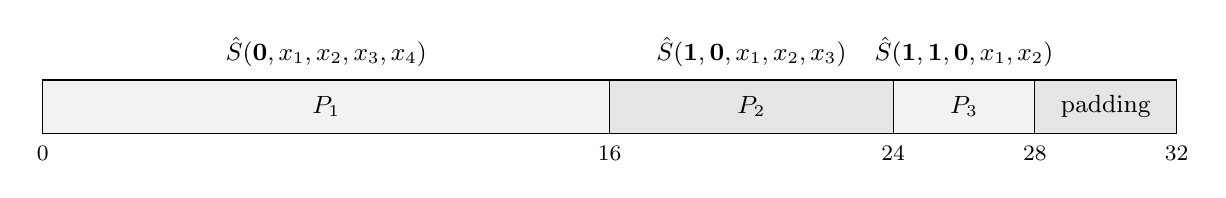
\begin{tikzpicture}[scale=0.45, every node/.style={font=\small}]
    \fill[gray!10] (0,0) rectangle (16,1.5);
    \fill[gray!20] (16,0) rectangle (24,1.5);
    \fill[gray!10] (24,0) rectangle (28,1.5);
    \fill[gray!20] (28,0) rectangle (32,1.5);

    \draw[black] (0,0) rectangle (32,1.5);
    \draw[black] (16,0) -- (16,1.5);
    \draw[black] (24,0) -- (24,1.5);
    \draw[black] (28,0) -- (28,1.5);

    \node at (8,0.75) {$P_1$};
    \node at (20,0.75) {$P_2$};
    \node at (26,0.75) {$P_3$};
    \node at (30,0.75) {padding};

    \node[below] at (0,-0.1) {\footnotesize 0};
    \node[below] at (16,-0.1) {\footnotesize 16};
    \node[below] at (24,-0.1) {\footnotesize 24};
    \node[below] at (28,-0.1) {\footnotesize 28};
    \node[below] at (32,-0.1) {\footnotesize 32};

    % Selector annotations above each section
    \node[above] at (8,1.6) {$\hat{S}({\mathbf{0}}, x_1, x_2, x_3, x_4)$};
    \node[above] at (20,1.6) {$\hat{S}({\mathbf{1}}, {\mathbf{0}}, x_1, x_2, x_3)$};
    \node[above] at (26,1.6) {$\hat{S}({\mathbf{1}}, {\mathbf{1}}, {\mathbf{0}}, x_1, x_2)$};
\end{tikzpicture}
\caption{Simple stacking of $P_1, P_2, P_3$ into a single vector $S$}
\label{fig:stacking}
\end{figure}

\subsection{Tables}\label{sec:table-sizes}

The execution trace is split across three \textit{tables}: \textsc{execution}, \textsc{extension}, and \textsc{poseidon}. Each table $T$ is a matrix of base-field elements, with a variable power-of-two height $2^{h_T}$, and a fixed number of columns $n_\text{column}^T = n_\text{shift}^T + n_\text{flat}^T$. Each column $\hat{\textsf{col}}^T_i$ ($i \in [0, n_\text{column}^T)$) is interpreted as a multilinear polynomial in ${h_T}$ variables.

We write $h_\textsc{exec}$, $h_\textsc{poseidon}$, $h_\textsc{extension}$ for the log-heights of the three tables, $h_\textsc{bytecode}$ for the bytecode log-size (so the bytecode has $2^{h_\textsc{bytecode}}$ instructions), and $h_\textsc{memory}$ for the memory log-size (so the memory has $2^{h_\textsc{memory}}$ cells).

Each VM cycle corresponds to a row of the $\textsc{EXECUTION}$, each poseidon precompile call corresponds to a row of the $\textsc{POSEIDON}$, and each extension precompile call with size parameter $N$ (\Cref{extension_op_instruction}) corresponds to $N$ rows of the $\textsc{EXTENSION}$ table.

We restrict their maximal heights, to ensure logup multiplicites never overflow modulo $p$:

\begin{center}
\begin{tabular}{lc}
\toprule
Table & Max rows \\
\midrule
\textsc{EXECUTION} & $2^{24}$ \\
\textsc{EXTENSION} & $2^{21}$ \\
\textsc{POSEIDON} & $2^{21}$ \\
\bottomrule
\end{tabular}
\end{center}

\subsection{One bus to interact between tables}\label{sec:bus-interactions}


In order for the tables (\Cref{sec:table-sizes}) to exchange data, we use a \emph{bus}: a global channel in which tables may \textsc{Push} or \textsc{Pull} tuples of $\textsf{bus\_width} = 16$ field elements in $\Fq$. We enforce the following property: \textit{every tuple is pulled exactly as many times as it is pushed}.

\subsubsection{Different types of interaction}

Every interaction is a tuple of $\textsf{bus\_width} = 16$ field elements with a fixed shape:
$$\sigma = \big(\,\underbrace{d_0,\ \dots,\ d_{N-1}}_{\text{data}},\quad \underbrace{0,\ \dots,\ 0}_{\text{padding}},\quad \textsf{domain\_sep}\,\big),$$

associated to a \emph{multiplicity}: a value $m \in \Fp$ counting the number of times that tuple is pushed (or pulled). The bus should be balanced: for every $\sigma$, the sums of all its \emph{push} multiplicities must equal the sum of all its \emph{pull} multiplicities.

The $N \le 15$ \emph{data} entries fill the low slots, the last slot always holds the \emph{domain separator} $\textsf{domain\_sep}$, and the slots in between are zero.



There are 4 different types of interactions:

\textbf{Memory:} Each memory fetch corresponds to a data pair $(\textsf{value}, \textsf{address})$, tagged with the domain separator $\textsf{memory\_sep} = 1$.

\textbf{Bytecode:} Each instruction fetch is the data tuple $(\textsf{instr}_0, \dots, \textsf{instr}_{11}, \textsf{pc})$, tagged with the domain separator $\textsf{bytecode\_sep} = 2$.

\textbf{Poseidon:} Each \textsc{POSEIDON} precompile call corresponds to a data tuple $(\nu_A, \nu_B, \nu_C)$ of its three memory pointers, tagged with a non-constant domain separator, that encodes some additional information (compression / permutation etc.), but which is an odd value $\ge 3$.

\textbf{Extension:} Each \textsc{EXTENSION} precompile call corresponds to a data tuple $(\nu_A, \nu_B, \nu_C)$ of its three memory pointers, tagged with a non-constant domain separator, that encodes some additional information (dot\_product / add / eq etc.), but which is a multiple of $4$.

\begin{center}
\begin{tabular}{lll}
\toprule
Kind & data entries & $\textsf{domain\_sep}$ \\
\midrule
Memory                   & $(\textsf{value},\ \textsf{address})$  & $\textsf{memory\_sep} = 1$ \\
Bytecode                 & $(\textsf{instr}_0,\ \dots,\ \textsf{instr}_{11},\ \textsf{pc})$ & $\textsf{bytecode\_sep} = 2$ \\
Poseidon     & $(\nu_A,\ \nu_B,\ \nu_C)$ & odd, $\ge 3$ \\
Extension & $(\nu_A,\ \nu_B,\ \nu_C)$ & multiple of $4$ \\
\bottomrule
\end{tabular}
\end{center}


A table $T$ may \textsc{Push} or \textsc{Pull} various tuples to the common bus.

\subsubsection{Special pushes for memory and bytecode}\label{sec:special-pushes}

Alongside committing to the execution trace (i.e.\ the table columns), the prover commits to two access-count multilinear polynomials:
\begin{itemize}
    \item $\textsf{memory\_acc} \in \Fp^{2^{h_\textsc{memory}}}$: $\textsf{memory\_acc}[i]$ = number of pulls of $(\textbf{m}[i], i, 0_{13}, \textsf{memory\_sep})$ across all tables.
    \item $\textsf{bytecode\_acc} \in \Fp^{2^{h_\textsc{bytecode}}}$: $\textsf{bytecode\_acc}[\textbf{pc}]$ = number of pulls of $(\textsf{instr}_0, \dots, \textsf{instr}_{11}, \textbf{pc}, 0_2, \textsf{bytecode\_sep})$ by the execution table.
\end{itemize}
These columns serve as the multiplicities of the two corresponding bus pushes:
\begin{itemize}
    \item For each $i \in [0, 2^{h_\textsc{memory}})$: $\textsc{Push}\big(\textbf{m}[i],\, i,\, 0_{13},\, \textsf{memory\_sep}\big)$ with multiplicity $\textsf{memory\_acc}[i]$.
    \item For each $\textbf{pc} \in [0, 2^{h_\textsc{bytecode}})$: $\textsc{Push}\big(\textsf{instr}_0(\textbf{pc}), \dots, \textsf{instr}_{11}(\textbf{pc}),\, \textbf{pc},\, 0_2,\, \textsf{bytecode\_sep}\big)$ with multiplicity $\textsf{bytecode\_acc}[\textbf{pc}]$.
\end{itemize}

\subsubsection{Balanced bus proved via logup}

\paragraph{Hashing tuples to a single field element.} For some $\vec\beta = (\beta_1, \ldots, \beta_\ell) \in \Fq^\ell$ sampled uniformly at random, we define:
\[
\pi_{\vec\beta}(\sigma) \;=\; \sum_{i=0}^{\textsf{bus\_width} - 1} \sigma_i \cdot \hat{eq}\big(\vec\beta,\, [i]_\text{bits}^\ell\big) \;=\; \hat{\sigma}(\vec\beta).
\]
By \Cref{lem:sz} applied to the (non-zero) multilinear polynomial $\hat\sigma - \hat{\sigma'}$ in $\ell$ variables, two distinct tuples collide with probability at most $\ell/q$.

\paragraph{Bus balance as a rational identity.} Enumerate the bus interactions across all tables as a list of pairs $(\sigma_k, m_k)_{1 \leq k \leq K}$, where $\sigma_k \in \Fp^{\textsf{bus\_width}}$ is the pushed (or pulled) tuple data and $m_k \in \Fp$ is its signed multiplicity (positive for \textsc{Push}, negative for \textsc{Pull}) (where we naturally embed the integers $(-p, p)$ into $\Fp$). Assume that, for every tuple $\sigma$, both the total pushes and the total pulls of $\sigma$ are strictly less than $p$. Then the bus is balanced if and only if, for every $\sigma$, $\sum_{k \,:\, \sigma_k = \sigma} m_k = 0$, which, for $\vec\beta \overset{\$}{\leftarrow} \Fq^\ell$ and $\gamma \overset{\$}{\leftarrow} \Fq$, is equivalent up to completeness error $K / q$ and soundness error $K \ell / q$ to:
\begin{equation} \label{eq:logup-sum}
\sum_{k=1}^{K} \frac{m_k}{\gamma - \pi_{\vec\beta}(\sigma_k)} \;=\; 0.
\end{equation}

\begin{proof}
(Inspired by \href{https://github.com/openvm-org/stark-backend/blob/main/docs/Soundness_of_Interactions_via_LogUp.pdf}{Soundness of Interactions via LogUp})
Define the $\Fp$-valued multiset $M(\sigma) = \sum_{k \,:\, \sigma_k = \sigma} m_k$, with support $S = \{\sigma : M(\sigma) \neq 0\}$, of size $s = |S|$. The bus is balanced iff $S = \emptyset$.

\emph{Completeness.} If $S = \emptyset$, then $M(\sigma) = 0$ for every $\sigma$, so the rational sum is identically zero wherever it is defined. The sum is undefined when $\gamma$ coincides with some pole $\pi_{\vec\beta}(\sigma_k)$, which over uniform $\gamma$ happens with probability at most $K/q$:  the protocol's \emph{completeness error}.

\emph{Soundness.} Suppose $S \neq \emptyset$, and define
\[
N(\vec\beta, \gamma) \;:=\; \sum_{\sigma \in S} M(\sigma) \prod_{\sigma' \in S \setminus \{\sigma\}}\!\big(\gamma - \pi_{\vec\beta}(\sigma')\big), \qquad Q(\vec\beta, \gamma) \;:=\; \prod_{\sigma \in S}\!\big(\gamma - \pi_{\vec\beta}(\sigma)\big).
\]
Over a common denominator, the rational sum equals $N/Q$. Verifier acceptance requires this fraction to be defined and equal to zero, hence forces $N(\vec\beta, \gamma) = 0$.

\emph{Total degree of $N$.} The degree of $N$, interpreted as multivariable polynomial in $\gamma$ and $\vec\beta$, is at most $(s-1)\ell \leq K \ell$.

\emph{Non-vanishing of $N$.} Pick any $\sigma^\star \in S$ (so $M(\sigma^\star) \neq 0$). To show $N$ is not the zero polynomial in $\Fq[\vec\beta, \gamma]$, substitute the variable $\gamma$ by the polynomial $\pi_{\vec\beta}(\sigma^\star) \in \Fq[\vec\beta]$. If $N$ were the zero polynomial its image would also be zero. For every $\sigma \in S$ with $\sigma \neq \sigma^\star$, the product $\prod_{\sigma' \in S \setminus \{\sigma\}}$ contains the factor $\gamma - \pi_{\vec\beta}(\sigma^\star)$ (since $\sigma^\star \in S \setminus \{\sigma\}$), which the substitution sends to $0$; only the $\sigma = \sigma^\star$ summand survives, giving
$$
N\big(\vec\beta,\, \pi_{\vec\beta}(\sigma^\star)\big) \;=\; M(\sigma^\star) \prod_{\sigma' \in S \setminus \{\sigma^\star\}} (\hat\sigma^\star - \hat\sigma')(\vec\beta) \;\in\; \Fq[\vec\beta].
$$
Each factor in this product is the MLE of the non-zero vector $\sigma^\star - \sigma' \in \Fp^{\textsf{bus\_width}}$, hence a non-zero polynomial in $\vec\beta$. Given that $M(\sigma^\star) \neq 0$, $N$ is non-zero in $\Fq[\vec\beta, \gamma]$.

By \Cref{lem:sz},
\[
\Pr_{\vec\beta, \gamma}[N(\vec\beta, \gamma) = 0] \;\leq\; K\,\ell/q. \qedhere
\]
\end{proof}

\subsubsection{Logup-GKR}

The prover can convince the verifier of the validity of \cref{eq:logup-sum} efficiently via GKR \cite{logup_gkr}, as long as the verifier can efficiently evaluate the MLEs of $(m_k)_{k \in [1, K]}$ and $(\pi_{\vec\beta}(\sigma_k))_{k \in [1, K]}$ (assuming $K$ is a power-of-two, which we can always guarantee up to some padding: zeros for numerators, ones for denominators).

We briefly recall the GKR construction in this context.

Assume the prover wants to convince the verifier $\sum_{b \in \{0, 1\}^n} \frac{\hat{num}(b)}{\hat{den}(b)} = \kappa$ for some $\hat{num}, \hat{den} \in \Fq^{<2}[X_1, \dots, X_n]$ efficiently evaluable and $\kappa \in \Fq$.

Define the following protocol $GKR(n):$

\begin{itemize}
    \item If $n = 0$, the verifier can evaluate the sum by evaluting $\hat{num} $ and $\hat{den}$ once each, at a common point (the empty point, since both are constant polynomial).
    \item If $n > 0:$ 
    \begin{itemize}
        \item Write $\kappa = \sum_{b \in \{0, 1\}^{n-1}} \frac{\hat{num}'(b)}{\hat{den}'(b)}$, where $num'$ is the MLE of $(\hat{num}(0, b) \cdot \hat{den}(1, b) + \hat{num}(1, b) \cdot \hat{den}(0, b))_{b \in \{0, 1\}^{n -1}}$ and $\hat{den}'$ is the MLE of $(\hat{den}(0, b) \cdot \hat{den}(1, b))_{b \in \{0, 1\}^{n -1}}$
        \item recursively call $GKR(n-1)$ on this new sum, which will return 2 claims of the form: $\hat{num}'(\alpha) = \beta^{num}$ and $\hat{den}'(\alpha) = \beta^{den}$ with $\alpha \in \Fq^{n-1}, \beta^{num}, \beta^{den}\in \Fq$.
        \item Sample $\gamma \in \Fq$ and run the sumcheck protocol on:
        $$\sum_{b \in \{0, 1\}^{n -1}} eq(\alpha, b)\big[(\hat{num}(0, b) \cdot \hat{den}(1, b) + \hat{num}(1, b) \cdot \hat{den}(0, b)) + \gamma \cdot \hat{den}(0, b) \cdot \hat{den}(1, b)\big] = \beta^{num} + \gamma \cdot \beta^{den}$$
        \item Let $\eta \in \Fq^{n-1}$ be the sumcheck challenges. The prover sends $num_0, num_1, den_0, den_1$, respectively equal to $\hat{num}(0, b), \hat{num}(1, b), \hat{den}(0, b), \hat{den}(1, b)$ in the honest case. This enables the verifier to evaluate the expression within the sum above, and to conclude the sumcheck.
        \item Sample $\delta \in \Fq$, and conclude the GKR step by outputing the following claims (that remains to be proven): $\hat{num}(\delta, \eta) \stackrel{?}{=} (1-\delta) \cdot num_0 + \delta \cdot num_1$ and $\hat{den}(\delta, \eta) \stackrel{?}{=} (1-\delta) \cdot den_0 + \delta \cdot den_1$.
    \end{itemize}
\end{itemize}

\subsubsection{Stacking within logup}

In practice, the fingerprinted data $\pi_{\vec\beta}(\sigma_k)$ and multiplicities $m_k$ come from multiple columns, of potentially different sizes. We stack them in a similar way than \Cref{sec:stacking}. TODO give more details

\subsection{AIR constraints}

Every table $T$ has a list of $n^\text{constraints}_T$ AIR (Algebraic Intermediate Representation) constraints. Each AIR constraint $C_k^T$ ($k \in [0, n_\text{constraints}^T)$) is a multivariate polynomial in $n_\text{column}^T + n_\text{shift}^T$ variables: one variable per column (taking its row-$r$ value $\textsf{col}^T_i(r)$ as input), plus one variable per shifted column (taking $\textsf{shift}(\textsf{col}^T_j)[r]$ as input). The constraint is respected by the table's trace if, for every row $r \in [0, 2^{h_T})$,
$$
C_k^T\big(\textsf{col}^T_0(r), \ldots, \textsf{col}^T_{n_\text{column}^T-1}(r),\ \textsf{shift}(\textsf{col}^T_0)[r], \ldots, \textsf{shift}(\textsf{col}^T_{n_\text{shift}^T-1})[r]\big) = 0.
$$

\subsubsection{ZeroCheck: Proving AIR constraints via sumcheck}

For each table $T$, we want to convince the verifier that every constraint $C_k^T$ vanishes on every row of the trace. We proceed in three steps.

\textbf{Batching.} The verifier samples a single $\mu \in \Fq$, and we form, for each table $T$, the batched constraint
\[
H_T \;:=\; \sum_{k=0}^{n_\text{constraints}^T - 1} \mu^{\iota_T + k}\, C_k^T,
\]
where $\iota_T := \sum_{T' < T} n_\text{constraints}^{T'}$ is the offset of $T$ in a global ordering of all constraints across all tables (so consecutive powers $1, \mu, \mu^2, \dots$ are distributed across all constraints).

\emph{Completeness}: if every $C_k^T$ vanishes on every row, so does each $H_T$.

\emph{Soundness}: if some $C_k^T$ fails to vanish at some row $\vec b^\star$, then $\mu \mapsto H_T(\vec b^\star)$ is a non-zero univariate polynomial of degree $< N := \sum_T n_\text{constraints}^T$, so $H_T(\vec b^\star) \neq 0$ except with soundness error $N/q$ over uniform $\mu$, via Schwartz-Zippel (\cref{lem:sz}).

\textbf{Zerocheck.} Let $f_T \in \Fq^{2^{h_T}}$ be the vector whose $\vec b$-th coordinate is
\[
f_T(\vec b) \;:=\; H_T\big(\hat{\textsf{col}}^T_0(\vec b), \ldots, \hat{\textsf{col}}^T_{n_\text{column}^T-1}(\vec b), \overset{\scriptscriptstyle\wedge}{\textsf{shift}}(\textsf{col}^T_0)(\vec b), \ldots, \overset{\scriptscriptstyle\wedge}{\textsf{shift}}(\textsf{col}^T_{n_\text{shift}^T-1})(\vec b)\big),
\]
so the claim is $f_T \equiv 0$. The verifier samples $\vec r \in \Fq^{h_T}$. By \Cref{lem:sz} applied to the multilinear polynomial (in $h_T$ variables) $\hat{f}_T$, with soundness error $h_T / q$ it suffices to prove that $\hat{f}_T(\vec r) = 0$, i.e.,
\[
\sum_{\vec b \in \{0,1\}^{h_T}} \hat{eq}(\vec b, \vec r) \cdot f_T(\vec b) \;=\; 0.
\]

\textbf{Sumcheck.} Run the standard sumcheck protocol \cite{sumcheck} on the sum above. After $h_T$ rounds with challenges $\vec\beta \in \Fq^{h_T}$, the verifier must check the summand at $\vec b = \vec\beta$: $\hat{eq}(\vec\beta, \vec r)$ is computed directly, and the column and shifted-column evaluations are claimed by the prover and verified as described in \Cref{sec:stacking}.

\textbf{Beyond consecutive sampling of the challenge $\vec r$.} Prover and verifier may engage in arbitrary auxiliary sub-protocols between successive $r_i$ samplings; what matters for soundness is only that each $r_i$ is sampled uniformly at random and after the trace commitment.

\subsubsection{Batching many ZeroChecks together}

Instead of running the zerocheck above individually for each table, we merge them into a single \emph{back-loaded} sumcheck of $h_{\max} := \max_T h_T$ rounds, using a shared random challenge $\vec r \in \Fq^{h_{\max}}$. For each table $T$, let $\vec r_T \in \Fq^{h_T}$ be the suffix of $\vec r$ of length $h_T$, write $\vec X_{\geq k} := (X_k, \ldots, X_{h_{\max} - 1})$, and define $G_T \in \Fq[X_0, \ldots, X_{h_{\max}-1}]$ by
\[
G_T(\vec X) \;:=\; \Big(\textstyle\prod_{i < h_{\max} - h_T} X_i\Big) \cdot \hat{eq}\big(\vec X_{\geq h_{\max} - h_T},\, \vec r_T\big) \cdot f_T\big(\vec X_{\geq h_{\max} - h_T}\big).
\]

We run a single sumcheck claiming
\[
\sum_{\vec b \in \{0, 1\}^{h_{\max}}} \sum_T G_T(\vec b) \;=\; 0,
\]
which is equivalent to the conjunction of the three per-table zerocheck claims.

\subsubsection{Attaching evaluation claims}\label{sec:air-eval}

Suppose, in addition to the AIR constraints, we also want to verify evaluation claims of the form $\hat{V}(\vec r_T) = v$, where $V$ is a polynomial expression in the columns of $T$ (sometimes called \emph{virtual column}, i.e. that is not committed). One way to see it: treat each such $V$ as just another constraint of $T$, batched in alongside the $C_k^T$'s with its own power of $\mu$ in the global ordering: the only difference is that its expected sum is no longer $0$. Listing all eval claims across the three tables as $(v_1, \dots, v_M)$ with respective global indices $(\iota_1, \dots, \iota_M)$, the zerocheck target shifts from $0$ to
\[
\sum_{i = 1}^{M} \mu^{\iota_i}\, v_i.
\]

\subsection{EXECUTION table}


\subsubsection{Columns}

 Each row corresponds to a VM cycle. It has $n_{cols}^{execution} = 20$ columns.

\begin{itemize}
    \item \textbf{pc} (program counter)
    \item \textbf{fp} (frame pointer)
    \item $\textsf{addr}_A$, $\textsf{addr}_B$, $\textsf{addr}_C$ (memory indexes)
    \item $\textsf{value}_A$, $\textsf{value}_B$, $\textsf{value}_C$ (corresponding memory values)
    \item 12 columns encoding the instruction being executed:
        \begin{itemize}
        \item $\textsf{flag}_A$, $\textsf{flag}_B$, $\textsf{flag}_C$, $\textsf{flag}^{C}_\textbf{fp}, \textsf{flag}_\textsf{mul}, \textsf{flag}_\textsf{jump}, \textsf{flag}^{AB}_\textbf{fp} \in \{0, 1\}$
        \item $\textsf{aux}_1 \in \{0, 1, 2\}$ ($\textsf{aux}_1$ handles both ADD and DEREF)
        \item $\textsf{operand}_A$, $\textsf{operand}_B$, $\textsf{operand}_C, \textsf{aux}_2 \in \Fp$
    \end{itemize}
\end{itemize}

\textbf{Note.} $\textsf{flag}^{AB}_\textbf{fp}$ is only used by precompile instructions; for ADD, MUL, DEREF, and JUMP it is always 0. We can reuse it to enrich the ISA. But is it worth it?


\subsubsection{Opcode encoding}\label{sec:opcode-encoding}

We first derive three values $\nu_A, \nu_B, \nu_C$ from the instruction columns:
\begin{itemize}
    \item $\nu_A = \textsf{flag}_A \cdot \textsf{operand}_A + (1 - \textsf{flag}_A - \textsf{flag}^{AB}_\textbf{fp}) \cdot \textsf{value}_A + \textsf{flag}^{AB}_\textbf{fp} \cdot (\textbf{fp} + \textsf{operand}_A)$
    \item $\nu_B = \textsf{flag}_B \cdot \textsf{operand}_B + (1 - \textsf{flag}_B - \textsf{flag}^{AB}_\textbf{fp}) \cdot \textsf{value}_B + \textsf{flag}^{AB}_\textbf{fp} \cdot (\textbf{fp} + \textsf{operand}_B)$
    \item $\nu_C = \textsf{flag}_C \cdot \textsf{operand}_C + (1 - \textsf{flag}_C - \textsf{flag}^{C}_\textbf{fp}) \cdot \textsf{value}_C + \textsf{flag}^{C}_\textbf{fp} \cdot (\textbf{fp} + \textsf{operand}_C)$
\end{itemize}

For an ISA operand pair $(x^\textsf{addr}, x) \in \{\texttt{imm}, \texttt{mem}, \texttt{fp\_rel}\} \times \Fp$ to be assigned to $\nu_X$ ($X \in \{A, B, C\}$), we write $\nu_X \!\leftarrow\! (x^\textsf{addr}, x)$ for the column assignment defined by
\[
\begin{array}{c|ll}
x^\textsf{addr} & \text{columns set} & \text{resulting }\nu_X \\
\hline
\texttt{imm} & \textsf{flag}_X = 1,\ \textsf{operand}_X = x & x \\
\texttt{mem} & \textsf{flag}_X = 0,\ \textsf{operand}_X = x & \textbf{m}[\textbf{fp} + x] \\
\texttt{fp\_rel} & \textsf{flag}^C_\textbf{fp} = 1,\ \textsf{operand}_C = x \quad (X = C \text{ only}) & \textbf{fp} + x
\end{array}
\]
For precompiles, when $\alpha^\textsf{addr} = \beta^\textsf{addr} = \texttt{fp\_rel}$, the encoding uses the simultaneous mode instead: $\textsf{flag}^{AB}_\textbf{fp} = 1$, $\textsf{operand}_A = \alpha$, $\textsf{operand}_B = \beta$, yielding $\nu_A = \textbf{fp} + \alpha$ and $\nu_B = \textbf{fp} + \beta$. All columns not explicitly set below are zero.

\begin{itemize}\setlength\itemsep{4pt}
    \item $\texttt{ADD}[\alpha^\textsf{addr}, \alpha, \beta^\textsf{addr}, \beta, \gamma^\textsf{addr}, \gamma]$ \; (semantics $\nu_A + \nu_C = \nu_B$): $\textsf{aux}_1 = 1$;\; $\nu_A \!\leftarrow\! (\alpha^\textsf{addr}, \alpha)$, $\nu_B \!\leftarrow\! (\beta^\textsf{addr}, \beta)$, $\nu_C \!\leftarrow\! (\gamma^\textsf{addr}, \gamma)$.
    \item $\texttt{MUL}[\alpha^\textsf{addr}, \alpha, \beta^\textsf{addr}, \beta, \gamma^\textsf{addr}, \gamma]$ \; (semantics $\nu_A \cdot \nu_C = \nu_B$): $\textsf{flag}_\textsf{mul} = 1$;\; $\nu_A \!\leftarrow\! (\alpha^\textsf{addr}, \alpha)$, $\nu_B \!\leftarrow\! (\beta^\textsf{addr}, \beta)$, $\nu_C \!\leftarrow\! (\gamma^\textsf{addr}, \gamma)$.
    \item $\texttt{DEREF}[\alpha, \beta, \gamma^\textsf{addr}, \gamma]$ \; (semantics $\textbf{m}[\textbf{m}[\textbf{fp} + \alpha] + \beta] = \nu_C$): $\textsf{aux}_1 = 2$;\; $\textsf{flag}_A = 0$, $\textsf{operand}_A = \alpha$ (so $\nu_A = \textbf{m}[\textbf{fp} + \alpha]$);\; $\textsf{flag}_B = 1$, $\textsf{operand}_B = \beta$;\; $\nu_C \!\leftarrow\! (\gamma^\textsf{addr}, \gamma)$.
    \item $\texttt{JUMP}[\alpha^\textsf{addr}, \alpha, \beta^\textsf{addr}, \beta, \gamma^\textsf{addr}, \gamma]$ \; (condition / dest / updated-fp): $\textsf{flag}_\textsf{jump} = 1$;\; $\nu_A \!\leftarrow\! (\alpha^\textsf{addr}, \alpha)$, $\nu_B \!\leftarrow\! (\beta^\textsf{addr}, \beta)$, $\nu_C \!\leftarrow\! (\gamma^\textsf{addr}, \gamma)$.
    \item $\texttt{POSEIDON\_OP}[\alpha^\textsf{addr}, \alpha, \beta^\textsf{addr}, \beta, \gamma^\textsf{addr}, \gamma, \texttt{permute}, \texttt{half}, \delta]$: \; $\nu_A \!\leftarrow\! (\alpha^\textsf{addr}, \alpha)$, $\nu_B \!\leftarrow\! (\beta^\textsf{addr}, \beta)$, $\nu_C \!\leftarrow\! (\gamma^\textsf{addr}, \gamma)$, and
    \[
    \textsf{aux}_2 = 3 + 2\,\texttt{permute} + 4\,\texttt{half} + 8\,[\delta \neq \bot] + 16\, \delta\,[\delta \neq \bot].
    \]
    \item $\texttt{EXTENSION\_OP}[\alpha^\textsf{addr}, \alpha, \beta^\textsf{addr}, \beta, \gamma^\textsf{addr}, \gamma, \texttt{op}, \textsf{flag\_be}, N]$: \; $\nu_A \!\leftarrow\! (\alpha^\textsf{addr}, \alpha)$, $\nu_B \!\leftarrow\! (\beta^\textsf{addr}, \beta)$, $\nu_C \!\leftarrow\! (\gamma^\textsf{addr}, \gamma)$, and
    \[
    \textsf{aux}_2 = 4\,\textsf{flag\_be} + 8\,\textsf{flag\_add} + 16\,\textsf{flag\_dot\_product} + 32\,\textsf{flag\_eq} + 64N,
    \]
    where $(\textsf{flag\_add}, \textsf{flag\_dot\_product}, \textsf{flag\_eq})$ is the one-hot encoding of $\texttt{op}$.
\end{itemize}


\subsubsection{AIR constraints}\label{sec:air-eval-after}

Constraints have degree 5. The values $\nu_A, \nu_B, \nu_C$ are as defined in \Cref{sec:opcode-encoding}.


Let $P_0, P_1, P_2$ be the Lagrange basis polynomials at $0, 1, 2$:
$$P_0(x) = (x-1)(x-2)/2, \qquad P_1(x) = x(2-x), \qquad P_2(x) = x(x-1)/2.$$
We define the virtual (non-committed) selectors
\begin{itemize}
    \item $\textsf{flag}_\textsf{add} = P_1(\textsf{aux}_1)$ \quad (equals $1$ when $\textsf{aux}_1 = 1$, else $0$ on $\{0, 2\}$),
    \item $\textsf{flag}_\textsf{deref} = P_2(\textsf{aux}_1)$ \quad (equals $1$ when $\textsf{aux}_1 = 2$, else $0$ on $\{0, 1\}$),
    \item $\textsf{flag}_\textsf{precompile} = 1 - (\textsf{flag}_\textsf{add} + \textsf{flag}_\textsf{mul} + \textsf{flag}_\textsf{deref} + \textsf{flag}_\textsf{jump})$.
\end{itemize}
$\textsf{flag}_\textsf{precompile}$ is the selector for the precompile bus push (see \Cref{sec:execution-bus}).

\paragraph{Addressing constraints.}
\begin{itemize}
    \item $(1 - \textsf{flag}_A - \textsf{flag}^{AB}_\textbf{fp}) \cdot (\textsf{address}_A - (\textbf{fp} + \textsf{operand}_A)) = 0$
    \item $(1 - \textsf{flag}_B - \textsf{flag}^{AB}_\textbf{fp}) \cdot (\textsf{address}_B - (\textbf{fp} + \textsf{operand}_B)) = 0$
    \item $(1 - \textsf{flag}_C - \textsf{flag}^{C}_\textbf{fp}) \cdot (\textsf{address}_C - (\textbf{fp} + \textsf{operand}_C)) = 0$
\end{itemize}


\paragraph{Per-opcode semantic constraints.}
\begin{itemize}
    \item $\texttt{ADD}$: $\quad \textsf{flag}_\textsf{add} \cdot (\nu_B - (\nu_A + \nu_C)) = 0$.
    \item $\texttt{MUL}$: $\quad \textsf{flag}_\textsf{mul} \cdot (\nu_B - \nu_A \cdot \nu_C) = 0$.
    \item $\texttt{DEREF}$: $\quad \textsf{flag}_\textsf{deref} \cdot (\textsf{addr}_B - (\textsf{value}_A + \textsf{operand}_B)) = 0$ \quad and \quad $\textsf{flag}_\textsf{deref} \cdot (\textsf{value}_B - \nu_C) = 0$.
    \item $\texttt{JUMP}$: let $J = \textsf{flag}_\textsf{jump} \cdot \nu_A$ (so $J = 1$ on a taken jump, $J = 0$ otherwise). Then:
    \begin{itemize}
        \item $J \cdot (1 - \nu_A) = 0$ \quad (forces $\nu_A \in \{0, 1\}$ on jump rows)
        \item $J \cdot (\text{next}(\textbf{pc}) - \nu_B) = 0$ \quad and \quad $(1 - J) \cdot (\text{next}(\textbf{pc}) - (\textbf{pc} + 1)) = 0$
        \item $J \cdot (\text{next}(\textbf{fp}) - \nu_C) = 0$ \quad and \quad $(1 - J) \cdot (\text{next}(\textbf{fp}) - \textbf{fp}) = 0$
    \end{itemize}
\end{itemize}

\paragraph{Well-formed-bytecode assumption.} The constraints above assume each instruction is well-formed.

TODO: Verify and (formally) prove completeness + soundness.

\subsubsection{Bus interactions}\label{sec:execution-bus}

\paragraph{Memory pulls (three per row).} For each $X \in \{A, B, C\}$:
\[
\textsc{Pull}\big(\textsf{value}_X,\, \textsf{addr}_X,\, 0_{13},\, \textsf{memory\_sep}\big) \quad \text{with multiplicity } 1.
\]

\paragraph{Bytecode pull (one per row).}
\[
\textsc{Pull}\big(\textsf{instr},\, \textbf{pc},\, 0_2,\, \textsf{bytecode\_sep}\big) \quad \text{with multiplicity } 1.
\]

where we write:
\[
\textsf{instr} \;=\; \big(\textsf{operand}_A, \textsf{operand}_B, \textsf{operand}_C, \textsf{flag}_A, \textsf{flag}_B, \textsf{flag}_C, \textsf{flag}^{C}_\textbf{fp}, \textsf{flag}^{AB}_\textbf{fp}, \textsf{flag}_\textsf{mul}, \textsf{flag}_\textsf{jump}, \textsf{aux}_1, \textsf{aux}_2\big)
\]
for the 12 instruction columns.

\paragraph{Precompile push (conditional).}
\[
\textsc{Push}\big(\nu_A,\, \nu_B,\, \nu_C,\, 0_{12},\, \textsf{aux}_2\big) \quad \text{with multiplicity } \textsf{flag}_\textsf{precompile} \text{ (see \Cref{sec:air-eval-after})},
\]
where $\textsf{aux}_2$ encodes a call to either the \textsf{POSEIDON} or \textsf{EXTENSION} table.

\subsection{POSEIDON table}

The Poseidon table runs one $\texttt{POSEIDON\_OP}$ precompile call (\Cref{sec:poseidon-op}) per row, pulling the call $(\nu_A, \nu_B, \nu_C, \textsf{aux}_2)$ from the precompile bus. The call's compile-time parameters $(\texttt{permute}, \texttt{half}, \delta)$ are recorded in the row as the boolean flags $\textsf{flag\_permute}, \textsf{flag\_short}, \textsf{flag\_left}$ and the offset $\textsf{offset\_left} \in \Fp$, with $\textsf{flag\_left} = [\delta \neq \bot]$ and $\textsf{offset\_left} = \delta$ (so $\textsf{flag\_left} = 1$ replaces the first four left-input elements by a hardcoded prefix, and $\textsf{flag\_short} = 1$ chops the compression output to its first four elements).

\subsubsection{Columns}

It has $n_{cols}^{poseidon} = 109$ columns.

\begin{itemize}
    \item \textbf{Control / pointers ($9$):} the multiplicity (for precompile bus-interaction) $\textsf{multiplicity}$ ($1$ on active rows, $0$ on padding); the boolean mode flags $\textsf{flag\_permute}$, $\textsf{flag\_short}$, $\textsf{flag\_left}$ and the offset $\textsf{offset\_left}$; the right-input and output pointers $\nu_B$, $\nu_C$; and two derived left addresses $\textsf{addr}^\text{lo}_\text{left}$, $\textsf{addr}^\text{hi}_\text{left}$, equal to $(\nu_A, \nu_A{+}4)$ if $\textsf{flag\_left}{=}0$ and to $(\textsf{offset\_left}, \nu_A)$ if $\textsf{flag\_left}{=}1$.
    \item \textbf{Input ($16$):} $\textsf{input}_0, \ldots, \textsf{input}_{15}$, the permutation input $\texttt{left} \,\|\, \texttt{right}$ (so $\textsf{input}_{0..8} = \texttt{left}$ and $\textsf{input}_{8..16} = \texttt{right}$).
    \item \textbf{Intermediate rounds ($68$):} the full state is committed only after each \emph{pair} of full rounds: $\textsf{full}_1, \textsf{full}_2$ ($16$ columns each) after the two pairs making up the $4$ initial full rounds, and $\textsf{full}_3$ ($16$ columns) after the first pair of the $4$ final full rounds (the last pair feeds the output columns directly). Plus $\textsf{sbox}_1, \ldots, \textsf{sbox}_{20}$, the single S-box output (the cube of the first state coordinate) committed at each partial round.
    \item \textbf{Output ($16$):} two halves $\textsf{out}_\text{lo}, \textsf{out}_\text{hi}$ ($8$ columns each). $\textsf{out}_\text{lo}$ holds the written first half — the feed-forward sum $s[0..8] + \texttt{left}$ in compression, or $s[0..8]$ in permutation; $\textsf{out}_\text{hi}$ holds $s[8..16]$ and is used only in permutation.
\end{itemize}

Non-committed (virtual): $\nu_A$ (left-input pointer) and $\textsf{aux}_2$ (the precompile-data domain separator, see below).

\subsubsection{Bus interactions}
\textbf{Memory pulls.} Each committed input/output cell is tied to memory by a $\textsc{Pull}\big(c,\, a,\, 0_{13},\, \textsf{memory\_sep}\big)$ of multiplicity $1$ (value $c$ at address $a$):
\begin{itemize}
    \item $\textsf{input}_i$ at $\textsf{addr}^\text{lo}_\text{left} + i$ and $\textsf{input}_{4+i}$ at $\textsf{addr}^\text{hi}_\text{left} + i$, for $i \in [0, 4)$ (the left half);
    \item $\textsf{input}_{8+i}$ at $\nu_B + i$, for $i \in [0, 8)$ (the right half);
    \item $\textsf{out}_\text{lo}[i]$ at $\nu_C + i$ and $\textsf{out}_\text{hi}[i]$ at $\nu_C + 8 + i$, for $i \in [0, 8)$.
\end{itemize}

\textbf{Precompile pull.} The table pulls the call tuple
\[
\textsc{Pull}\big(\nu_A,\, \nu_B,\, \nu_C,\, 0_{12},\, \textsf{aux}_2\big) \quad \text{with multiplicity } \textsf{multiplicity},
\]
matching the push issued by the execution table (\Cref{sec:execution-bus}), with domain separator
\[
\textsf{aux}_2 = 3 + 2\,\textsf{flag\_permute} + 4\,\textsf{flag\_short} + 8\,\textsf{flag\_left} + 16\,\textsf{flag\_left} \cdot \textsf{offset\_left}
\]
packing all three flags and the offset. This encoding is injective: the flags are boolean (AIR-enforced), and when $\textsf{flag\_left} = 1$ the left lookup forces $\textsf{offset\_left} < 2^{h_\textsc{memory}} \leq 2^{26} < p/2$, so no wrap-around occurs modulo $p$; when $\textsf{flag\_left} = 0$, $\textsf{offset\_left}$ does not enter $\textsf{aux}_2$.

\subsubsection{AIR constraints}

Constraints have degree $10$.

Write $\nu_A = \textsf{addr}^\text{hi}_\text{left} - (1 - \textsf{flag\_left}) \cdot 4$ for the (virtual) left-input pointer, and let $\sigma \in \Fp^{16}$ denote the running state of the recomputed permutation.

\textbf{Booleanity ($4$).} $\textsf{multiplicity}$, $\textsf{flag\_permute}$, $\textsf{flag\_short}$, $\textsf{flag\_left}$ are each boolean: $x \cdot (1 - x) = 0$.

\textbf{Mode separation ($1$).} $\textsf{flag\_permute} \cdot (\textsf{flag\_short} + \textsf{flag\_left}) = 0$  (permutation excludes the two compression optimizations)

\textbf{Left-address binding ($2$).}
\begin{itemize}
    \item $\textsf{flag\_left} \cdot (\textsf{offset\_left} - \textsf{addr}^\text{lo}_\text{left}) = 0$ \quad (when $\textsf{flag\_left} = 1$: $\textsf{addr}^\text{lo}_\text{left} = \textsf{offset\_left}$, $\textsf{addr}^\text{hi}_\text{left} = \nu_A$);
    \item $(1 - \textsf{flag\_left}) \cdot (\nu_A - \textsf{addr}^\text{lo}_\text{left}) = 0$ \quad (when $\textsf{flag\_left} = 0$: $\textsf{addr}^\text{lo}_\text{left} = \nu_A$, $\textsf{addr}^\text{hi}_\text{left} = \nu_A + 4$).
\end{itemize}

\textbf{Permutation ($68$).} Starting from $\sigma = \textsf{input}$, recompute the Poseidon permutation (round constants, S-box $x \mapsto x^3$, and the MDS / sparse partial-round layers; we omit the Poseidon-internal details), and check it against the committed round witnesses:
\begin{itemize}
    \item \emph{full-round pairs ($48$):} after each committed pair, the $16$ recomputed coordinates equal the witness — $\sigma = \textsf{full}_1$, then $\textsf{full}_2$ (the two initial pairs), then $\textsf{full}_3$ (the first final pair);
    \item \emph{partial rounds ($20$):} at partial round $k$, $\textsf{sbox}_k = (\sigma_0)^3$ (and $\sigma_0$ is then set to $\textsf{sbox}_k$, keeping the constraint low-degree).
\end{itemize}

\textbf{Output ($24$).} Let $\sigma$ be the state after the \emph{last} (uncommitted) final full-round pair, and set the gates $g_i = 1 - \textsf{flag\_permute}$ for $i \in [0,4)$ and $g_i = 1 - \textsf{flag\_permute} - \textsf{flag\_short}$ for $i \in [4,8)$. For each $i \in [0, 8)$:
\begin{itemize}
    \item $g_i \cdot \big(\sigma_i + \textsf{input}_i - \textsf{out}_\text{lo}[i]\big) = 0$ \quad (compression: feed-forward sum, with the upper half gated off when $\textsf{flag\_short} = 1$);
    \item $\textsf{flag\_permute} \cdot \big(\sigma_i - \textsf{out}_\text{lo}[i]\big) = 0$ \quad and \quad $\textsf{flag\_permute} \cdot \big(\sigma_{i+8} - \textsf{out}_\text{hi}[i]\big) = 0$ \quad (permutation: raw output).
\end{itemize}


\subsection{EXTENSION table}

\subsubsection{Trace layout}

Each extension field operation occupies $N$ consecutive rows, where $N$ is the length parameter of the $\texttt{EXTENSION\_OP}$ instruction (the number of element pairs in the dot product / sum / eq operation, see \Cref{extension_op_instruction}): one row per element pair, with the column $\textsf{len}$ counting down from $N$ on the first row to $1$ on the last. Within a group, rows are ordered from first element to last, but the \textsf{acc} column accumulates backward: the first row holds the full result, the last row holds only the final element's value. Padding rows have all operation flags set to 0 and $\textsf{flag\_start} = 1$, $\textsf{len} = 1$.

\vspace{3mm}

\noindent\resizebox{\textwidth}{!}{%
\begin{tabular}{ccccccccccccccc}
\toprule
\textsf{flag\_be} & \textsf{flag\_start} & $\textsf{flag\_add}$ & $\textsf{flag\_dot\_product}$ & $\textsf{flag\_eq}$ & \textsf{len} & $\textsf{idx}_A$ & $\textsf{idx}_B$ & $\textsf{idx}_R$ & $v_A$ \tiny{(5 columns)} & $v_B$ \tiny{(5 columns)} & \textsf{res} \tiny{(5 columns)} & \textsf{acc} \tiny{(5 columns)} & & $\textsf{aux}_2$ \\
\midrule
\multicolumn{15}{l}{\textit{DOT\_PRODUCT, base $\times$ extension, $N\!=\!4$ ($\nu_A\!=\!90$, $\nu_B\!=\!211$, $\nu_C\!=\!74$): \quad $\textsf{res} = \sum_{i=0}^{3} \textbf{m}[90\!+\!i] \cdot \textbf{m}[211\!+\!5i..216\!+\!5i]$}} \\[2pt]
1 & 1 & 0 & 1 & 0 & 4 & 90  & 211 & 74 & $\textbf{m}[90..95]$  & $\textbf{m}[211..216]$ & $\textbf{m}[74..79]$ & $e_0\!+\!e_1\!+\!e_2\!+\!e_3$ & & 276 \\
1 & 0 & 0 & 1 & 0 & 3 & 91  & 216 & 74 & $\textbf{m}[91..96]$  & $\textbf{m}[216..221]$ & $\textbf{m}[74..79]$ & $e_1\!+\!e_2\!+\!e_3$       & & 212 \\
1 & 0 & 0 & 1 & 0 & 2 & 92  & 221 & 74 & $\textbf{m}[92..97]$  & $\textbf{m}[221..226]$ & $\textbf{m}[74..79]$ & $e_2\!+\!e_3$               & & 148 \\
1 & 0 & 0 & 1 & 0 & 1 & 93  & 226 & 74 & $\textbf{m}[93..98]$  & $\textbf{m}[226..231]$ & $\textbf{m}[74..79]$ & $e_3$                       & & 84  \\
\midrule
\multicolumn{15}{l}{\textit{ADD, extension $\times$ extension, $N\!=\!3$ ($\nu_A\!=\!400$, $\nu_B\!=\!500$, $\nu_C\!=\!300$): \quad $\textsf{res} = \sum_{i=0}^{2} (\textbf{m}[400\!+\!5i..405\!+\!5i] + \textbf{m}[500\!+\!5i..505\!+\!5i])$}} \\[2pt]
0 & 1 & 1 & 0 & 0 & 3 & 400 & 500 & 300 & $\textbf{m}[400..405]$ & $\textbf{m}[500..505]$ & $\textbf{m}[300..305]$ & $e_0\!+\!e_1\!+\!e_2$ & & 200 \\
0 & 0 & 1 & 0 & 0 & 2 & 405 & 505 & 300 & $\textbf{m}[405..410]$ & $\textbf{m}[505..510]$ & $\textbf{m}[300..305]$ & $e_1\!+\!e_2$         & & 136 \\
0 & 0 & 1 & 0 & 0 & 1 & 410 & 510 & 300 & $\textbf{m}[410..415]$ & $\textbf{m}[510..515]$ & $\textbf{m}[300..305]$ & $e_2$                 & & 72 \\
\midrule
\multicolumn{15}{l}{\textit{EQ, extension $\times$ extension, $N\!=\!3$ ($\nu_A\!=\!600$, $\nu_B\!=\!700$, $\nu_C\!=\!800$): \quad $\textsf{res} = \prod_{i=0}^{2} [a_i b_i + (1\!-\!a_i)(1\!-\!b_i)]$}} \\[2pt]
0 & 1 & 0 & 0 & 1 & 3 & 600 & 700 & 800 & $\textbf{m}[600..605]$ & $\textbf{m}[700..705]$ & $\textbf{m}[800..805]$ & $e_0 \cdot e_1 \cdot e_2$ & & 224 \\
0 & 0 & 0 & 0 & 1 & 2 & 605 & 705 & 800 & $\textbf{m}[605..610]$ & $\textbf{m}[705..710]$ & $\textbf{m}[800..805]$ & $e_1 \cdot e_2$           & & 160 \\
0 & 0 & 0 & 0 & 1 & 1 & 610 & 710 & 800 & $\textbf{m}[610..615]$ & $\textbf{m}[710..715]$ & $\textbf{m}[800..805]$ & $e_2$                     & & 96 \\
\midrule
\multicolumn{15}{l}{\textit{Padding row}} \\[2pt]
0 & 1 & 0 & 0 & 0 & 1 & 0   & 0   & 0   & $\textbf{m}[0..5]$ & $\textbf{m}[0..5]$ & $\textbf{m}[0..5]$ & 0 & & 64 \\
\bottomrule
\end{tabular}%
}

\subsubsection{Columns}

There are 29 columns. Extension field values are represented as 5 consecutive columns.

\vspace{2mm}

\begin{itemize}
    \item \textsf{flag\_be} $\in \{0,1\}$: mode flag (1: base $\times$ extension, 0: extension $\times$ extension)
    \item \textsf{flag\_start} $\in \{0,1\}$: group boundary (1 on first row of each group and on padding, 0 elsewhere)
    \item $\textsf{flag\_add}$, $\textsf{flag\_dot\_product}$, $\textsf{flag\_eq}$ $\in \{0,1\}$: operation selectors (exactly one is 1 on active rows, all 0 on padding)
    \item \textsf{len}: countdown from $N$ to 1 within each group (1 on padding)
    \item $\textsf{idx}_A$, $\textsf{idx}_B$, $\textsf{idx}_R$: memory addresses of the two operands and of the result
    \item $v_A = (v_A[0], \dots, v_A[4])$ (5 columns): the 5 base field values claimed to live at memory addresses $\textsf{idx}_A, \dots, \textsf{idx}_A + 4$ (enforced by the memory pulls below). In extension $\times$ extension mode, $v_A$ is interpreted as the extension field element $\mathsf{embed}(v_A)$; in base $\times$ extension mode, only $v_A[0]$ is used (as a base field scalar) and the remaining coordinates $v_A[1..5]$ are unconstrained.
    \item $v_B = (v_B[0], \dots, v_B[4])$ (5 columns): same as $v_A$ at addresses $\textsf{idx}_B, \dots, \textsf{idx}_B + 4$; always interpreted as the extension field element $\mathsf{embed}(v_B)$.
    \item $\textsf{res} = (\textsf{res}[0], \dots, \textsf{res}[4])$ (5 columns): the 5 base field values of the output extension field element, claimed to live at addresses $\textsf{idx}_R, \dots, \textsf{idx}_R + 4$. Constant on all rows of a group.
    \item $\textsf{acc} = (\textsf{acc}[0], \dots, \textsf{acc}[4])$ (5 columns): running accumulator (over $\Fq$) of the per-element contributions $e_\bullet$ defined in the AIR constraints below; on \textsf{flag\_start} rows it equals $\textsf{res}$.
\end{itemize}

Virtual (non-committed) columns: $\textsf{multiplicity} = \textsf{flag\_start} \cdot (\textsf{flag\_add} + \textsf{flag\_dot\_product} + \textsf{flag\_eq})$ and $\textsf{aux}_2 = 4 \cdot \textsf{flag\_be} + 8 \cdot \textsf{flag\_add} + 16 \cdot \textsf{flag\_dot\_product} + 32 \cdot \textsf{flag\_eq} + 64 \cdot \textsf{len}$

\subsubsection{Bus interactions}

\textbf{Memory pulls.} For each operand $(s, \textsf{idx}) \in \{(v_A, \textsf{idx}_A),\, (v_B, \textsf{idx}_B),\, (\textsf{res}, \textsf{idx}_R)\}$ and each $k \in [0, 5)$:
\[
\textsc{Pull}\big(s[k],\, \textsf{idx} + k,\, 0_{13},\, \textsf{memory\_sep}\big) \quad \text{with multiplicity } 1.
\]

\textbf{Precompile pull.}
\[
\textsc{Pull}\big(\textsf{idx}_A,\, \textsf{idx}_B,\, \textsf{idx}_R,\, 0_{12},\, \textsf{aux}_2\big) \quad \text{with multiplicity } \textsf{multiplicity},
\]
The domain separator $\textsf{aux}_2$ binds the mode and length to the bus data: since $\textsf{flag\_be}, \textsf{flag\_add}, \textsf{flag\_dot\_product}, \textsf{flag\_eq}$ are boolean and the length is $\leq 2^{21}$ (\Cref{lem:len-bound}), the encoding is injective, so every $\textsf{aux}_2$ sent by the execution table is faithfully received here.


\subsubsection{AIR constraints}

We use AIR constraints of degree 6.

\vspace{2mm}

Let $\tilde v_A = (v_A[0],\, (1 - \textsf{flag\_be}) \cdot v_A[1],\, \dots,\, (1 - \textsf{flag\_be}) \cdot v_A[4])$, and define the per-element (virtual) results
\[
    e_\text{add} = \tilde v_A + v_B, \qquad e_\text{dot\_product} = \tilde v_A \cdot v_B, \qquad e_\text{eq} = \tilde v_A \cdot v_B + (1 - \tilde v_A)(1 - v_B),
\]
where sums and products are in $\Fq = \Fp[X]/(X^5 + X^2 - 1)$ (\Cref{sec:field}). Each $e_\bullet$ is therefore a 5-tuple of base field expressions (one per coordinate), and each coordinate-valued constraint below stands for 5 base field constraints.

Let $\textsf{acc\_tail} = \text{next}(\textsf{acc}) \cdot (1 - \text{next}(\textsf{flag\_start}))$.

\vspace{2mm}

\textbf{Boolean flags.} Each of $\textsf{flag\_be}, \textsf{flag\_start}, \textsf{flag\_add}, \textsf{flag\_dot\_product}, \textsf{flag\_eq}$ is constrained to be boolean:
\begin{itemize}
    \item \refstepcounter{equation}\textbf{(\theequation)}\label{c:bool-flags}\hspace{1mm} $f \cdot (1 - f) = 0$ for $f \in \{\textsf{flag\_be},\, \textsf{flag\_start},\, \textsf{flag\_add},\, \textsf{flag\_dot\_product},\, \textsf{flag\_eq}\}$.
\end{itemize}

\textbf{Per-row accumulation and result.} The running accumulator $\textsf{acc}$ propagates the per-element contribution backwards:
\begin{itemize}
    \item $\textsf{flag\_add} \cdot (\textsf{acc} - e_\text{add} - \textsf{acc\_tail}) = 0$ \hfill (ADD: additive accumulation)
    \item $\textsf{flag\_dot\_product} \cdot (\textsf{acc} - e_\text{dot\_product} - \textsf{acc\_tail}) = 0$ \hfill (DOT\_PRODUCT: additive accumulation)
    \item $\textsf{flag\_eq} \cdot (\textsf{acc} - e_\text{eq} \cdot (\textsf{acc\_tail} + \text{next}(\textsf{flag\_start}))) = 0$ \hfill (EQ: multiplicative accumulation)
    \item $\textsf{flag\_start} \cdot (\textsf{acc} - \textsf{res}) = 0$ \hfill (on group-start rows, $\textsf{acc} = \textsf{res}$)
\end{itemize}

\textbf{Intra-group consistency.} Within a group (i.e.\ when the next row is not a group start), the mode/operation flags are constant, $\textsf{len}$ counts down by 1, and the input pointers advance by their natural stride (1 base field cell for $\textsf{idx}_A$ in base $\times$ extension mode, 5 cells otherwise):
\begin{itemize}
    \item \refstepcounter{equation}\textbf{(\theequation)}\label{c:len-countdown}\hspace{1mm} $(1 - \text{next}(\textsf{flag\_start})) \cdot (\textsf{len} - \text{next}(\textsf{len}) - 1) = 0$ \hfill ($\textsf{len}$ countdown)
    \item $(1 - \text{next}(\textsf{flag\_start})) \cdot (f - \text{next}(f)) = 0$ for $f \in \{\textsf{flag\_be},\, \textsf{flag\_add},\, \textsf{flag\_dot\_product},\, \textsf{flag\_eq}\}$ \hfill (mode/operation constant)
    \item $(1 - \text{next}(\textsf{flag\_start})) \cdot (\text{next}(\textsf{idx}_A) - \textsf{idx}_A - (\textsf{flag\_be} + (1 - \textsf{flag\_be}) \cdot 5)) = 0$ \hfill ($\textsf{idx}_A$ stride)
    \item $(1 - \text{next}(\textsf{flag\_start})) \cdot (\text{next}(\textsf{idx}_B) - \textsf{idx}_B - 5) = 0$ \hfill ($\textsf{idx}_B$ stride)
\end{itemize}

\textbf{Group boundary.} When the next row starts a new group, the current group must have reached its last element:
\begin{itemize}
    \item \refstepcounter{equation}\textbf{(\theequation)}\label{c:len-boundary}\hspace{1mm} $\text{next}(\textsf{flag\_start}) \cdot (\textsf{len} - 1) = 0$ \hfill ($\textsf{len} = 1$ on the last row of a group)
\end{itemize}

\vspace{5mm}

\begin{lemma}\label{lem:len-bound}
On every row $r$ of the extension table, $\textsf{len}_r \leq H - r$ (as an integer in $\{0, \dots, p-1\}$), where $H \leq 2^{21}$ is the table height. In particular, $\textsf{len}_r \leq H$.
\end{lemma}

\begin{proof}
By backward induction on $r$, from $r = H - 1$ down to $r = 0$.

\vspace{2mm}

\textbf{Base case ($r = H - 1$):} On the wrapping pair (row $H\!-\!1$ paired with itself, see \Cref{sec:next-mle}), $\text{next}(x) = x$ for every column $x$. Constraint~\eqref{c:len-countdown} becomes $(1 - \textsf{flag\_start}) \cdot (\textsf{len} - \textsf{len} - 1) = -(1 - \textsf{flag\_start}) = 0$, forcing $\textsf{flag\_start}_{H-1} = 1$ (which is itself in $\{0, 1\}$ by~\eqref{c:bool-flags} applied to $f = \textsf{flag\_start}$). Then \eqref{c:len-boundary} becomes $1 \cdot (\textsf{len} - 1) = 0$, giving $\textsf{len}_{H-1} = 1 = H - (H-1)$.

\vspace{2mm}

\textbf{Inductive step ($r < H - 1$):} Assume $\textsf{len}_s \leq H - s$ for all $s > r$. The pair (row $r$, row $r\!+\!1$) gives two cases depending on $\textsf{flag\_start}_{r+1} \in \{0,1\}$ (by~\eqref{c:bool-flags} applied to $f = \textsf{flag\_start}$):

\begin{itemize}
    \item If $\textsf{flag\_start}_{r+1} = 1$: \eqref{c:len-boundary} gives $1 \cdot (\textsf{len}_r - 1) = 0$, so $\textsf{len}_r = 1 \leq H - r$.
    \item If $\textsf{flag\_start}_{r+1} = 0$: \eqref{c:len-countdown} gives $(1 - 0) \cdot (\textsf{len}_r - \textsf{len}_{r+1} - 1) = 0$, so $\textsf{len}_r = \textsf{len}_{r+1} + 1$ in $\Fp$. By induction, $\textsf{len}_{r+1} \leq H - (r+1)$, so $\textsf{len}_{r+1} + 1 \leq H - r$. Since $H - r \leq H \leq 2^{21} < p$, the addition does not overflow modulo $p$, so $\textsf{len}_r = \textsf{len}_{r+1} + 1 \leq H - r$ as integers.
\end{itemize}
\end{proof}

\vspace{3mm}

TODO: Verify and (formally) prove soundness.

\subsection{End-to-end protocol}\label{sec:e2e-protocol}


\vspace{2mm}

\noindent\fbox{%
\begin{minipage}{0.97\textwidth}
\textbf{Verification parameters (known to both prover and verifier).}
\begin{itemize}
    \item $\textsf{bytecode}$: the bytecode of the program being executed (\Cref{sec:opcode-encoding}), of size $2^{h_\textsc{bytecode}}$.
    \item $\textsf{public\_input}$: the initial public part of the memory, occupying cells $[0,\, \ell_\textsc{public})$ with $\ell_\textsc{public} = 8$.
\end{itemize}
\end{minipage}}

\vspace{3mm}

\begin{enumerate}
    \item \textbf{Dimensions.} 
    The prover sends $(\textsf{log\_inv\_rate},\, h_\textsc{memory},\, h_\textsc{exec},\, h_\textsc{poseidon},\, h_\textsc{extension})$.
    
    The verifier checks: $\textsf{log\_inv\_rate}^{\min} \leq \textsf{log\_inv\_rate} \leq \textsf{log\_inv\_rate}^{\max}$ (i.e.\ $1 \leq \textsf{log\_inv\_rate} \leq 4$); $h^{\min} \leq h_T \leq h_T^{\max}$ for each $T \in \{\textsc{exec}, \textsc{poseidon}, \textsc{extension}\}$ (\Cref{sec:table-sizes}); $h_\textsc{memory}^{\min} \leq h_\textsc{memory} \leq h_\textsc{memory}^{\max}$; $h_\textsc{bytecode} \geq h^{\min}$; and $h_\textsc{memory} \geq \max(h_\textsc{bytecode},\, h_\textsc{exec},\, h_\textsc{poseidon},\, h_\textsc{extension})$.

    \item \textbf{Stacked commitment.} The prover commits via WHIR \cite{whir} to a single multilinear polynomial stacking (see \Cref{sec:stacking}) the memory $\textbf{m}$, the access counts $\textsf{memory\_acc}$ and $\textsf{bytecode\_acc}$, and all committed columns of the three tables.

    \item \textbf{Logup.}
    \begin{enumerate}
        \item  The verifier samples $\gamma \in \Fq$ and $\vec\beta \in \Fq^{\ell}$ (bus-tuple hashing seeds, $\ell = \log_2 \textsf{bus\_width}$), used for \Cref{eq:logup-sum}.
        \item  Run the GKR protocol of \Cref{sec:bus-interactions} to compute the sum of quotients from \Cref{eq:logup-sum}. The sum contains terms from: the memory section ($2^{h_\textsc{memory}}$ entries) and the bytecode section ($\max(2^{h_\textsc{bytecode}}, 2^{h_\textsc{exec}})$ entries, padded if $h_\textsc{bytecode} < h_\textsc{exec}$; see \Cref{sec:special-pushes}), then, for each table $T$ sorted by descending height, one block of $2^{h_T}$ entries per bus interaction of $T$. Write $h_\textsc{gkr}$ for the log2-ceiling of the resulting total length.

        The protocol yields a point $\vec r_\textsc{gkr} \in \Fq^{h_\textsc{gkr}}$ and two scalar claims $(e_\text{num}, e_\text{den})$ on the numerator and denominator MLEs at $\vec r_\textsc{gkr}$.

         \item The prover sends, at the appropriate suffixes of $\vec r_\textsc{gkr}$:
    \begin{itemize}
        \item the evaluations of $\textsf{memory\_acc}$ and $\textbf{m}$ for the memory section;
        \item the evaluation of $\textsf{bytecode\_acc}$ for the bytecode section;
        \item for each table $T$ and each bus interaction of $T$, the per-column evaluations needed to reconstruct that bus's numerator/denominator contribution.
    \end{itemize}
    The verifier recombines these evaluations into a claimed total numerator and denominator and checks they equal $(e_\text{num}, e_\text{den})$.
    \end{enumerate}

    \item \textbf{AIR.}
    \begin{enumerate}
        \item The verifier samples $\mu \in \Fq$. Consecutive powers $1, \mu, \mu^2, \dots$ are used to take a random linear combination of \emph{all} verification constraints across the three tables.
        \item Prover and verifier run the back-loaded batched zerocheck of \Cref{sec:air-eval}, merging the per-table constraint polynomials into a single sumcheck of $h_\textsc{max} := \max_T h_T$ rounds, \emph{crucially reusing the suffix of $\vec r_\textsc{gkr}$ of length $h_\textsc{max}$ from the logup step as the zerocheck random challenge (no fresh point is sampled)}. TODO explain why do this, and TODO explain why it's sound. Let $\vec r_\textsc{air} \in \Fq^{h_\textsc{max}}$ denote the sumcheck challenges.
        \item For each table $T$, the prover sends the evaluations of all of $T$'s committed columns and shifted columns at the appropriate suffix of $\vec r_\textsc{air}$. The verifier evaluates $T$'s AIR-constraint polynomial at these column evaluations, which enables to conclude the batched-zerocheck.
    \end{enumerate}

    \item \textbf{Public-memory consistency.} The verifier samples $\vec r_\textsc{pub} \in \Fq^{\log_2 \ell_\textsc{public}}$ and evaluates $\textsf{public\_input}$ as a multilinear polynomial at $\vec r_\textsc{pub}$, obtaining $v_\textsc{pub} \in \Fq$. The pair $(\vec r_\textsc{pub}, v_\textsc{pub})$ is queued as an opening claim on the initial $\ell_\textsc{public}$-cell prefix of the committed memory polynomial (handled by WHIR below).

    \item \textbf{Boundary pc.} To ensure a valid initial / final program counter, we add two opening claims on the \textbf{pc} column of the \textsc{execution} table: $\hat{\textbf{pc}}(0, \ldots, 0) = 0$ and $\hat{\textbf{pc}}(1, \ldots, 1) = 2^{h_\textsc{bytecode}} - 1$ (handled by WHIR bellow).

    \item \textbf{WHIR opening.} The prover and verifier run a single WHIR verification on the stacked commitment of step~2 against the list of evaluation claims (including shifted ones) gathered so far.

\end{enumerate}

\subsection{Fiat-Shamir}

In order to turn the interactive protocol described in \Cref{sec:e2e-protocol} into a non-interactive one, we apply the BCS transformation \cite{BCS}. In particular, we use the Fiat-Shamir transformation implemented via a duplex sponge \cite{fiat_shamir_duplex_sponge} (using the $\texttt{POSEIDON}^\pi$ permutation over a state of 16 KoalaBear field elements).

\section{ISA programming}

This section describes \emph{conventions} for writing programs using the ISA of \Cref{sec:isa}. None of it is hard-coded into the VM or enforced by the snark.

\subsection{Hints}\label{sec:hints}

A \emph{hint} is the use of non-determinism: the prover supplies a value, the program then verifies it, in order to replace an expensive computation by a cheap check.

\begin{exmp} Computing an inverse $y := x^{-1} \in \Fp$. $y$ is hinted to some memory cell and the program performs the single check $x \cdot y = 1$: one MUL.
\end{exmp}

% \paragraph{Sorting.} Sorting an array $a$ of length $n$ from scratch costs $O(n \log n)$ comparisons (see \Cref{sec:range-checks}). We can instead hint a candidate sorted array $b$ \emph{together with} a list of indices $\pi(0), \dots, \pi(n-1) \in [0, n)$ claiming that $b[i] = a[\pi(i)]$. The program then only has to verify
% \begin{enumerate}
%     \item $b$ is non-decreasing: one comparison per adjacent pair, $n-1$ in total.
%     \item $b[i] = a[\pi(i)]$ for every $i \in [0, n)$: $n$ memory reads.
%     \item $\pi(i) < n$ for every $i \in [0, n)$: one range check per index (\Cref{sec:range-checks}).
%     \item $\pi$ is injective. Take a pointer $\textsf{scratch} \in [0, 2^{h_\textsc{memory}} - n)$ to a fresh memory segment of size $n$. For each $i \in [0, n)$, write $\textbf{m}[\textsf{scratch} + \pi(i)] = i$. Any collision $\pi(i) = \pi(j)$ with $i \neq j$ would force the same cell to take two different values, breaking the write-once invariant and invalidating the trace. Combined with step~3, $\pi : [0, n) \to [0, n)$ is then a bijection, hence a permutation.
% \end{enumerate}
% All four checks are $O(n)$, beating the $\Theta(n \log n)$ of an in-program sort.

\subsection{Functions}\label{sec:functions}

A \emph{function} is a piece of bytecode, associated to:
\begin{itemize}
    \item a starting $\textbf{pc}$
    \item a number of inputs $n_\textsf{in}$
    \item a number of outputs $n_\textsf{out}$
    \item a frame size $s \geq 2 + n_\textsf{in} + n_\textsf{out}$ (in memory)
\end{itemize}
Every call operates on a fresh contiguous block of $s$ memory cells: its \emph{frame}, pointed to by $\textbf{fp}$ during execution. By convention, this frame contains the following data:
\begin{center}
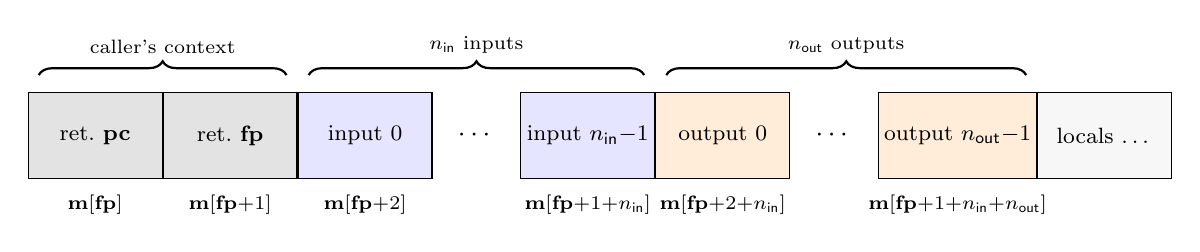
\begin{tikzpicture}[
    cell/.style={draw, minimum width=1.7cm, minimum height=1.1cm, font=\footnotesize, inner sep=2pt},
    ctxcell/.style={cell, fill=gray!22},
    incell/.style={cell, fill=blue!10},
    outcell/.style={cell, fill=orange!15},
    loccell/.style={cell, fill=gray!6},
    brace/.style={decorate, decoration={brace, amplitude=5pt, raise=2pt}, thick}
]
    % memory cells
    \node[ctxcell] (c0) at (0, 0) {ret.\ $\textbf{pc}$};
    \node[ctxcell, right=0pt of c0] (c1) {ret.\ $\textbf{fp}$};
    \node[incell, right=0pt of c1] (i0) {input $0$};
    \node[right=0pt of i0, draw=none, minimum width=1.1cm] (idots) {$\cdots$};
    \node[incell, right=0pt of idots] (iN) {input $n_\textsf{in}{-}1$};
    \node[outcell, right=0pt of iN] (o0) {output $0$};
    \node[right=0pt of o0, draw=none, minimum width=1.1cm] (odots) {$\cdots$};
    \node[outcell, right=0pt of odots] (oN) {output $n_\textsf{out}{-}1$};
    \node[loccell, right=0pt of oN] (loc) {locals \dots};

    % address labels below each cell
    \node[below=2pt of c0,  font=\scriptsize] {$\textbf{m}[\textbf{fp}]$};
    \node[below=2pt of c1,  font=\scriptsize] {$\textbf{m}[\textbf{fp}{+}1]$};
    \node[below=2pt of i0,  font=\scriptsize] {$\textbf{m}[\textbf{fp}{+}2]$};
    \node[below=2pt of iN,  font=\scriptsize] {$\textbf{m}[\textbf{fp}{+}1{+}n_\textsf{in}]$};
    \node[below=2pt of o0,  font=\scriptsize] {$\textbf{m}[\textbf{fp}{+}2{+}n_\textsf{in}]$};
    \node[below=2pt of oN,  font=\scriptsize] {$\textbf{m}[\textbf{fp}{+}1{+}n_\textsf{in}{+}n_\textsf{out}]$};

    % top braces (slightly inset on each side so adjacent braces don't touch)
    \draw[brace] ([yshift=4pt, xshift=4pt]c0.north west) -- ([yshift=4pt, xshift=-4pt]c1.north east) node[midway, above=6pt, font=\scriptsize] {caller's context};
    \draw[brace] ([yshift=4pt, xshift=4pt]i0.north west) -- ([yshift=4pt, xshift=-4pt]iN.north east) node[midway, above=6pt, font=\scriptsize] {$n_\textsf{in}$ inputs};
    \draw[brace] ([yshift=4pt, xshift=4pt]o0.north west) -- ([yshift=4pt, xshift=-4pt]oN.north east) node[midway, above=6pt, font=\scriptsize] {$n_\textsf{out}$ outputs};
\end{tikzpicture}
\end{center}

\textbf{Call.} Say the caller is at $\textbf{pc} = \textbf{pc}_\text{caller}$, $\textbf{fp} = \textbf{fp}_\text{caller}$, about to invoke a function $f$ with entry point $\textbf{pc}_f$ and inputs $a_0, \dots, a_{n_\textsf{in}-1}$ (either constants or memory cells). It obtains a hinted frame pointer $\textbf{fp}_\text{callee}$ (supposedly pointing to a fresh interval of size $s$ in memory) and executes:
\begin{itemize}
    \item $\textbf{m}[\textbf{fp}_\text{callee}] \gets \textbf{pc}_\text{ret}$, where $\textbf{pc}_\text{ret}  = \textbf{pc}_\text{caller} + 2 + n_\textsf{in}$ is the address of the instruction following the JUMP below;
    \item $\textbf{m}[\textbf{fp}_\text{callee} + 1] \gets \textbf{fp}_\text{caller}$;
    \item $\textbf{m}[\textbf{fp}_\text{callee} + 2 + k] \gets a_k$ for $k = 0, \dots, n_\textsf{in} - 1$;
    \item JUMP with $\textbf{pc} \gets \textbf{pc}_f$ and $\textbf{fp} \gets \textbf{fp}_\text{callee}$.
\end{itemize}

\textbf{Return.} Before returning, the callee has written its $n_\textsf{out}$ outputs $r_0, \dots, r_{n_\textsf{out}-1}$ to $\textbf{m}[\textbf{fp} + 2 + n_\textsf{in} + k] \gets r_k$ for $k = 0, \dots, n_\textsf{out} - 1$. It then executes the JUMP $\textbf{pc} \gets \textbf{m}[\textbf{fp}]$, $\textbf{fp} \gets \textbf{m}[\textbf{fp} + 1]$, which reads back $\textbf{pc}_\text{ret}$ and $\textbf{fp}_\text{caller}$. Execution resumes at $\textbf{pc}_\text{ret}$ in the caller's original frame.

\paragraph{No allocation pointer.} Cairo \cite{cairo} keeps a register $\textbf{ap}$ pointing to the next free memory cell. leanVM does not: the write-once memory (\Cref{sec:memory}) prevents any frame from overwriting previously-written data. And since a function's internal logic should only depend on its inputs, not on where its frame happens to land, the exact value of $\textbf{fp}_\text{callee}$ does not matter to the verifier.


\subsection{Loops}\label{sec:loops}

We suggest to unroll loops when the number of iterations is low, and known at compile time.

The remaining loops are transformed into recursive functions (by a compiler):

\begin{exmp}
Summing the $n$ entries of an array $a$:

\begin{center}
\begin{minipage}[t]{0.46\textwidth}
\centering\textit{loop form}
\begin{verbatim}
sum(a, n):
    s = 0
    for i in [0, n):
        s = s + a[i]
    return s
\end{verbatim}
\end{minipage}
\hfill
\begin{minipage}[t]{0.46\textwidth}
\centering\textit{recursive form}
\begin{verbatim}
sum(a, n):
    return sum_rec(a, n, 0, 0)

sum_rec(a, n, i, s):
    if i == n:
        return s
    return sum_rec(a, n, i + 1, s + a[i])
\end{verbatim}
\end{minipage}
\end{center}

\end{exmp}

\subsection{Range checks}\label{sec:range-checks}

It's possible to check that a memory cell is smaller than $t$ (for $t \leq 2^{16}$) in 3 cycles, where $t$ is either a constant or a memory cell \footnote{This idea was pointed out by D. Khovratovich, and is an unplanned use of the DEREF instruction}.

In case $t$ is a memory cell, the program should crucially enforce $t \leq 2^{16}$ (potentially using, again, a range check).

We denote by \textbf{m}[\textbf{fp} + $x$] the memory cell for which we want to ensure \textbf{m}[\textbf{fp} + $x$] $< t$.
We also denote by \textbf{m}[\textbf{fp} + $i$], \textbf{m}[\textbf{fp} + $j$] and \textbf{m}[\textbf{fp} + $k$] 3 auxiliary memory cells (that have not been used yet).
\begin{enumerate}
    \item \textbf{m}[\textbf{m}[\textbf{fp} + $x$]] = \textbf{m}[\textbf{fp} + $i$] (using DEREF, this ensures \textbf{m}[\textbf{fp} + $x$] $ < M$, the memory size)
    \item \textbf{m}[\textbf{fp} + $x$] + \textbf{m}[\textbf{fp} + $j$] = (t-1) (using ADD, this computes $\textbf{m}[\textbf{fp} + $j$] = t - 1 - $ \textbf{m}[\textbf{fp} + $x$])
        \item \textbf{m}[\textbf{m}[\textbf{fp} + $j$]] = \textbf{m}[\textbf{fp} + $k$] (using DEREF, this ensures $t - 1 - $ \textbf{m}[\textbf{fp} + $x$] $ < M$)
\end{enumerate}

Given $t \leq 2^{16} \leq 2^{h_\textsc{memory}}$, \textbf{m}[\textbf{fp} + $x$] $< 2^{h_\textsc{memory}}$, $t - 1 - $ \textbf{m}[\textbf{fp} + $x$] $< 2^{h_\textsc{memory}}$, and $2^{h_\textsc{memory}} \leq 2^{26} < p / 2$, we have: \textbf{m}[\textbf{fp} + $x$] $ < t$.

Note: From the point of view of the prover running the program: filling the values of \textbf{m}[\textbf{fp} + $i$] and \textbf{m}[\textbf{fp} + $k$] must be done at end of execution.


\begin{exmp}
	Let's say we want to write a function with 2 arguments $x = \textbf{m}$[\textbf{fp} + 2] and $y = \textbf{m}$[\textbf{fp} + 3] ($\textbf{m}$[\textbf{fp} + 0] and $\textbf{m}$[\textbf{fp} + 1] are used, by convention, to store the caller's \textbf{pc} and \textbf{fp}, to return to the previous context at the end of the function), which perform the following:
	
	\begin{enumerate}
		\item assert(x $<$ 10)
		\item z := x*y + 100
		\item assert(z $<$ 1000)
	\end{enumerate}
	
	Which can be compiled to:
	
	\begin{enumerate}
		\item \textbf{m}[\textbf{fp} + 4] = \textbf{m}[\textbf{m}$\big[$\textbf{fp} + 2$\big]$] // check that $x$ is "small"
		\item \textbf{m}[\textbf{fp} + 2] + \textbf{m}[\textbf{fp} + 5] = 9 // compute $9 - x$
		\item \textbf{m}[\textbf{fp} + 6] = \textbf{m}[\textbf{m}$\big[$\textbf{fp} + 5$\big]$] // check that $9 - x$ is "small"
		\item \textbf{m}[\textbf{fp} + 7] = \textbf{m}[\textbf{fp} + 2] * \textbf{m}[\textbf{fp} + 3] // compute $x.y$
		\item \textbf{m}[\textbf{fp} + 8] = \textbf{m}[\textbf{fp} + 7] + 100 // compute $z = x.y + 100$
		\item \textbf{m}[\textbf{fp} + 9] = \textbf{m}[\textbf{m}$\big[$\textbf{fp} + 8$\big]$] // check that $z$ is "small"
		\item \textbf{m}[\textbf{fp} + 8] + \textbf{m}[\textbf{fp} + 10] = 999 // compute $999 - z$
		\item \textbf{m}[\textbf{fp} + 11] = \textbf{m}[\textbf{m}$\big[$\textbf{fp} + 10$\big]$] // check that $999 - z$ is "small"
		\item JUMP with next(\textbf{pc}) = \textbf{m}[\textbf{fp} + 0], next(\textbf{fp}) = \textbf{m}[\textbf{fp} + 1], condition = 1 // return
	\end{enumerate}
	
	 
\end{exmp}


\subsection{Switch statements}

A switch dispatches to one of $k$ different code blocks based on a runtime value $x$ known to satisfy $0 \leq x < k$ (if $x$ came from a hint, it must be range-checked first; see \Cref{sec:range-checks}).

Implementation: place the $k$ blocks at regular intervals in the bytecode, all of the same length $b$ (the smaller blocks are padded with unreachable instructions), starting at $\textbf{pc} = a$ (the block for $x = 0$). The dispatch is then a single JUMP to $\textbf{pc} = a + b \cdot x$.

\begin{exmp}
Computing the $x$-th decimal digit of $\pi = 3.1415\dots$ for $x \in \{0, 1, 2, 3\}$:
\[
    r \;=\; \begin{cases} 3 & x = 0 \\ 1 & x = 1 \\ 4 & x = 2 \\ 1 & x = 3 \end{cases}
\]

\begin{framed}
\small
\begin{verbatim}
   ;; dispatch (a = 100, b = 2, x = m[fp+3])
   97: MUL[imm, 2,    mem, 4,   mem, 3]      ; m[fp+4] = 2 * x
   98: ADD[imm, 100,  mem, 5,   mem, 4]      ; m[fp+5] = 100 + 2*x
   99: JUMP[imm, 1,   mem, 5,   fp_rel, 0]   ; pc <- m[fp+5]

   ;; 4 blocks, each of length b = 2, laid out at regular intervals
  100: ADD[imm, 3,    mem, 6,   imm, 0]      ; res = 3         
  101: JUMP[imm, 1,   imm, 108, fp_rel, 0]   ; pc <- 108     

  102: ADD[imm, 1,    mem, 6,   imm, 0]      ; res = 1        
  103: JUMP[imm, 1,   imm, 108, fp_rel, 0]   ; pc <- 108   

  104: ADD[imm, 4,    mem, 6,   imm, 0]      ; res = 4        
  105: JUMP[imm, 1,   imm, 108, fp_rel, 0]   ; pc <- 108    

  106: ADD[imm, 1,    mem, 6,   imm, 0]      ; res = 1         
  107: JUMP[imm, 1,   imm, 108, fp_rel, 0]   ; pc <- 108   

  108: ...                                                       ;; merge
\end{verbatim}
\end{framed}

\end{exmp}

\subsection{Compiling from a high-level zkDSL}\label{sec:zkdsl-to-ssa}

A high-level zkDSL (with mutable variables, loops, and conditionals) can be compiled to the ISA, by systematically translating mutation into \emph{Static Single-Assignment} (SSA) form, and every loop by a recursive function (\Cref{sec:loops}).

\begin{exmp}
\begin{framed}
\small
\noindent
\begin{minipage}[t]{0.42\textwidth}
\textit{source}
\begin{verbatim}
def func(n):
    x: Mut = 1
    x += 2
    x = x * 4
    for i in range(0, n):
        x += i
    return x
\end{verbatim}
\end{minipage}%
\begin{minipage}[t]{0.46\textwidth}
\textit{after an intial compilation pass}
\begin{verbatim}
def func(n):
    x1 = 1
    x2 = x1 + 2
    x3 = x2 * 4
    x_buff = Array(n + 1)
    x_buff[0] = x3
    loop(0, n, x_buff)
    return x_buff[n]

def loop(i, n, x_buff):
    if i == n:
        return
    x_buff[i+1] = x_buff[i] + i
    loop(i + 1, n, x_buff)
\end{verbatim}
\end{minipage}
\end{framed}
Here $\textsf{Array}(k)$ is a hint: a prover-supplied pointer to a fresh region of $k$ memory cells.
\end{exmp}


\section{Signature aggregation}\label{sec:signature-aggregation}

XMSS \cite{ethereum_signatures} is a stateful hash-based signature scheme: each signature is bound to a nonce $s$. Aggregated via leanVM, XMSS is a promising candidate as a Post-Quantum replacement for BLS \cite{bls} at the consensus layer of Ethereum.

\paragraph{Statement we prove.} Fix a slot $s$, a message $\textsf{msg}$ and a list of public keys $\textsf{pk}_1, \dots, \textsf{pk}_K$. In Ethereum Consensus' setting, $s$ is the current consensus slot and $\textsf{msg}$ is the block hash. The aggregation proof attests knowledge soundness of:
\[
    \exists\, \sigma_1, \dots, \sigma_K \;\;\text{such that}\;\; \textsf{XMSS.Verify}(\textsf{pk}_k,\, \textsf{msg},\, s,\, \sigma_k) = \textsc{true} \quad \text{for every } k \in [1, K].
\]
The proof's public input is $(s,\, \textsf{msg},\, \textsf{pk}_1, \dots, \textsf{pk}_K)$; the individual signatures are part of the witness.

We need to support recursive aggregation: being able to further aggregate a list of previously aggregated signatures.

\begin{figure}[ht]
\centering
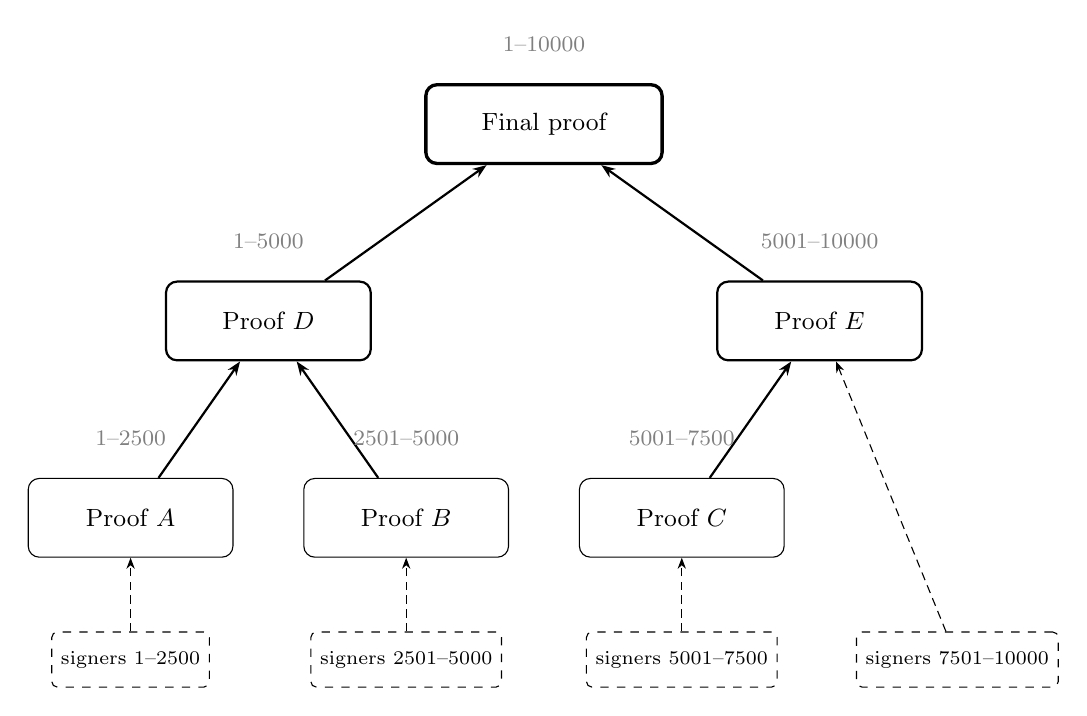
\begin{tikzpicture}[
    proof/.style={draw, rounded corners=4pt, minimum width=2.6cm, minimum height=1cm, align=center, font=\small},
    leaf/.style={proof},
    merge/.style={proof, line width=0.8pt},
    root/.style={proof, minimum width=3cm, line width=1.2pt},
    xmss/.style={draw, dashed, rounded corners=2pt, minimum width=1.6cm, minimum height=0.7cm, align=center, font=\scriptsize},
    attests/.style={font=\footnotesize, text=black!50},
    arr/.style={-{Stealth[length=5pt]}, thick},
    sigarr/.style={-{Stealth[length=4pt]}, densely dashed, thin},
]

% --- XMSS signature blocks (inputs) ---
\node[xmss] (S1) at (0, -1.8) {signers $1$--$2500$};
\node[xmss] (S2) at (3.5, -1.8) {signers $2501$--$5000$};
\node[xmss] (S3) at (7, -1.8) {signers $5001$--$7500$};
\node[xmss] (S4) at (10.5, -1.8) {signers $7501$--$10000$};

% --- Leaf proofs ---
\node[leaf] (L1) at (0, 0) {Proof $A$};
\node[leaf] (L2) at (3.5, 0) {Proof $B$};
\node[leaf] (L3) at (7, 0) {Proof $C$};

% XMSS -> leaf arrows
\draw[sigarr] (S1) -- (L1);
\draw[sigarr] (S2) -- (L2);
\draw[sigarr] (S3) -- (L3);

% --- Middle level ---
\node[merge] (M1) at (1.75, 2.5) {Proof $D$};
\node[merge] (M2) at (8.75, 2.5) {Proof $E$};

% XMSS -> E (direct group)
\draw[sigarr] (S4) -- (M2);

% Recursive arrows: leaves -> middle
\draw[arr] (L1) -- (M1);
\draw[arr] (L2) -- (M1);
\draw[arr] (L3) -- (M2);

% --- Root ---
\node[root] (R) at (5.25, 5) {Final proof};

% Recursive arrows: middle -> root
\draw[arr] (M1) -- (R);
\draw[arr] (M2) -- (R);

% --- Coverage annotations (above each proof) ---
\node[attests, above=8pt of L1] {$1\text{--}2500$};
\node[attests, above=8pt of L2] {$2501\text{--}5000$};
\node[attests, above=8pt of L3] {$5001\text{--}7500$};
\node[attests, above=8pt of M1] {$1\text{--}5000$};
\node[attests, above=8pt of M2] {$5001\text{--}10000$};
\node[attests, above=8pt of R] {$1\text{--}10000$};

\end{tikzpicture}
\caption{Example of recursive aggregation of 10000 XMSS, sharing a common message. (Note: overlapping sets of signers are possible.) }
\label{fig:recursive-aggregation}
\end{figure}


\subsection{Recursive Aggregation}\label{sec:recursive-aggregation}

The recursive aggregation program (see \Cref{fig:recursive-aggregation}) attests that a set of public keys have valid signatures for a given message. It partitions the signers into $n_{\text{rec}} + 1$ sources: one \textbf{direct source} whose XMSS signatures are verified explicitly, and $n_{\text{rec}} \geq 0$ \textbf{recursive sources}, each accompanied by a sub-proof that is recursively verified.


\begin{framed}
\small
\begin{verbatim}
def aggregate(slot, msg, pks):       # msg:message, pks: public keys

    # the prover partitions pks into 1 direct subset + n_rec recursive subsets
    direct = hint()                  # subset of pks to verify directly
    n_rec  = hint()                  # number of recursive groups
    groups = hint()                  # groups[j] = subset of pks for j = 0..n_rec-1

    for pk in direct:
        sig = hint()
        assert XMSS.Verify(pk, msg, slot, sig)

    for j in range(n_rec):
        sub_proof = hint()
        assert leanVM.Verify(
            bytecode      = THIS_PROGRAM,  # self-dependency, see section below
            public_input  = (slot, msg, groups[j]),
            proof         = sub_proof,
        )

    # every pk in pks must appear in direct or in some groups[j]
    assert_full_coverage(pks, direct, groups)
\end{verbatim}
\end{framed}

\subsubsection{Bytecode evaluation claims}\label{sec:bytecode-reduction}

A key subtlety arises from recursion. Every leanVM proof is tied to a specific \emph{bytecode} --- the program that was executed, represented as a multilinear polynomial. In our case, there is a single program (that contains both the signature verification and recursion algorithms). The leanVM verification algorithm requires evaluating the bytecode polynomial at a random point.

When the recursive aggregation program verifies a sub-proof, it runs the leanVM verifier \emph{inside} the program. This verification produces a bytecode evaluation claim. For efficiency, rather than checking it inside the program (with a PCS), the claim is forwarded to the public input, to be checked externally.

However, each sub-proof is potentially itself a recursive aggregation, and may have already forwarded its own bytecode claim in the same way. So for each of the $n_{\text{rec}}$ sub-proofs, \textbf{two} bytecode claims arise:

\begin{enumerate}
    \item \textbf{Inner-public-memory claim}: The bytecode claim that the sub-proof forwarded from its own recursive verifications (read from the sub-proof's public input).

    \item \textbf{Inner-proof claim}: The new bytecode claim produced by verifying the sub-proof itself.
\end{enumerate}

After verifying all $n_{\text{rec}}$ sub-proofs, a fresh Fiat--Shamir transcript is initialized and fed with all $2 n_{\text{rec}}$ evaluation points and claimed values. This transcript produces a random linear combination challenge, and the $2 n_{\text{rec}}$ claims are then batched into a single one via sumcheck, yielding a reduced claim. This reduced claim is written to the public input for the next level of recursion.

When $n_{\text{rec}} = 0$ (no recursion), the bytecode claim in the public input is set to zero.


\subsubsection{Signer partitioning}\label{sec:signer-partitioning}

\emph{
In the following, we assume  the message being signed is common to all signers (typically the case at Ethereum's consensus layer), but the scheme can be naturally adapted to distinct messages.}

\vspace{3mm}

Consider an aggregation of $n_{\text{sigs}}$ (distinct) signatures. The $n_{\text{sigs}}$ (distinct) public keys are part of the "public input" in memory. The aggregation program must ensure that each public key is verified by at least one of the $1 + n_{\text{rec}}$ sources (duplications allowed: some public keys may be verified by multiple sources).

Let $n_{\text{dup}}$ be the total number of duplicated public keys across sources, counted with multiplicity. To ensure valid partitioning, we use the following algorithm:

\begin{itemize}
    \item Initialize a counter $c \gets 0$.
    \item Initialize a (write-once) array $B$ of size $n_{\text{total}} = n_{\text{sigs}} + n_{\text{dup}}$.
    \item For each source $s$, for each signature index $i \in [0, n_{\text{total}})$ verified by $s$, write $B[i] \gets c$ and increment $c$.
    \item At the end, assert $c = n_{\text{total}}$.
\end{itemize}


\clearpage
\appendix

\section{WHIR \cite{whir} Optimizations}


\subsection{Avoid paying for (most of) the zero suffix from polynomial stacking}\label{sec:zero-suffix}

The polynomial $S$ (in $\nu$ variables) committed by WHIR (using an interleaved Reed-Solomon code) is the \emph{stacking} (\Cref{sec:stacking}) of all columns, memory, and access counts, padded with zeros up to the next power of two; its $2^\nu$ evaluations are therefore non-zero only on a prefix of some length $L$ ($2^{\nu - 1} < L \leq 2^\nu$). The first WHIR round folds $X_1, \ldots, X_{f_0^\text{whir}}$ (where $f_0^\text{whir} = 7$ is the initial folding factor), which splits the evaluations (on the boolean hypercube) of $S$ into $2^{f_0^\text{whir}} = 128$ contiguous blocks. Each block is Reed-Solomon encoded, and the $128$ encoded blocks become the columns of a matrix whose rows are the Merkle leaves.

Because the folded variables are the \emph{most significant} bits, the zeros land in the last blocks: only the first $n_\text{eff} = \lceil L / 2^{\nu - f_0^\text{whir}} \rceil$ blocks are non-zero, so every leaf ends with the same $128 - n_\text{eff}$ zeros. Two optimizations follow:

\begin{itemize}
    \item \textbf{FFT:} only the first $n_\text{eff}$ blocks are FFT encoded (trailing zero blocks encode to zero)
    \item \textbf{Leaf hashing:} we hash each Merkle leaf via a sponge absorbing data right-to-left, so the shared zero suffix yields the same partial state, which we precompute once and reuse for every leaf.
\end{itemize}

\subsection{Small-Value Optimization (SVO) and Split-Eq}\label{sec:svo}

WHIR opening contains a sumcheck of the form $\sum_{b \in \{0,1\}^\nu} w(b)\, f(b)$, where $f$ is the committed (base-field) polynomial and the weight $w(b) = \sum_i \alpha^i\, \hat{eq}(b, w_i)$ batches the evaluation claims $f(w_i) = y_i$ (we omit 'shift' claims for simplicity, but this is generalizable). In our setting the claims are highly \emph{sparse}: stacking many table columns into a single WHIR instance produces, for each column, a claim $w_i$ whose high-order coordinates are the boolean prefix bits selecting that column, with only the remaining coordinates in $\Fq$.

The \emph{small-value optimization} (SVO), together with the \emph{split-eq} trick (algo. 6 of \cite{Speeding-Up-Sum-Check-Proving}), speeds up the first $\ell_0$  sumcheck rounds (where most of the prover's cost lies) by precomputing accumulators (via the factorization $\hat{eq}(b, w_i) = \hat{eq}(b^{lo}, w_i^{lo}) \cdot \hat{eq}(b^{hi}, w_i^{hi})$). For prover cost to be proportional to the \emph{non-sparse} part of each claim, the boolean (sparse) coordinates must sit at the \emph{opposite end} from the variables folded first.

This conflicts with the zero-suffix optimization of \Cref{sec:zero-suffix}, which folds the \emph{most significant} variables first ($X_1, X_2, \dots$). TODO can we (efficiently) reconcile the 2 optimizations?

\clearpage
\bibliographystyle{IEEEtran}
\bibliography{bibliography}

\end{document}